\documentclass[11pt,a4paper]{article}

% ── Packages ──
\usepackage[margin=0.85in,headheight=15pt,top=0.8in,bottom=0.9in]{geometry}
\usepackage{cite}
\usepackage{amsmath,amssymb,amsfonts,amsthm}
\usepackage{algorithmic}
\usepackage{algorithm}
\usepackage{graphicx}
\usepackage{textcomp}
\usepackage{xcolor}
\usepackage{booktabs}
\usepackage{multirow}
\usepackage{array}
\usepackage{tabularx}
\usepackage{url}
\usepackage{hyperref}
\usepackage{listings}
\usepackage{subcaption}
\usepackage{enumitem}
\usepackage{setspace}
\usepackage{titlesec}
\usepackage{fancyhdr}
\usepackage{float}
\usepackage{pgfplots}
\pgfplotsset{compat=1.18}
\usepgfplotslibrary{statistics}

% Clickable, colored hyperlinks for citations and URLs
\hypersetup{
  colorlinks=true,
  linkcolor=blue!60!black,
  citecolor=blue!60!black,
  urlcolor=blue!70!black,
  pdftitle={Fast PUF-Based Authentication Protocol for UAV Swarm Networks},
  pdfauthor={Md Ziyad Hussain}
}

\newtheorem{theorem}{Theorem}
\newtheorem{lemma}[theorem]{Lemma}
\newtheorem{definition}{Definition}

\setstretch{1.05}

% Compact section spacing
\titlespacing*{\section}{0pt}{1.2ex plus 0.4ex minus 0.2ex}{0.6ex plus 0.2ex}
\titlespacing*{\subsection}{0pt}{0.9ex plus 0.3ex minus 0.2ex}{0.4ex plus 0.2ex}
\titlespacing*{\subsubsection}{0pt}{0.6ex plus 0.2ex minus 0.1ex}{0.3ex plus 0.1ex}
\setlist{itemsep=1pt, topsep=2pt, parsep=1pt}

\lstset{
  basicstyle=\ttfamily\small,
  breaklines=true,
  frame=single,
  numbers=left,
  numberstyle=\tiny,
  captionpos=b
}

\pagestyle{fancy}
\fancyhf{}
\rhead{\thepage}
\lhead{Fast Authentication Between UAVs}
\renewcommand{\headrulewidth}{0.4pt}

\begin{document}

% ══════════════════════════════════════════════════════════════
% TITLE PAGE
% ══════════════════════════════════════════════════════════════
\begin{titlepage}
\centering
\vspace*{0.4cm}

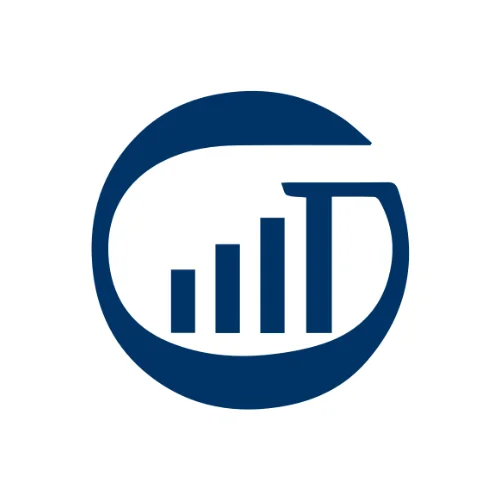
\includegraphics[width=2.6cm]{image.png}

\vspace{0.6cm}

{\LARGE \textbf{Indian Institute of Information Technology Guwahati}}

\vspace{0.2cm}

{\large Department of Computer Science and Engineering}

\vspace{1.6cm}

{\Huge \textbf{Fast Authentication Between UAVs}}

\vspace{0.5cm}

{\large A Technical Report on PUF-Based Swarm Authentication with OMNeT++ Simulation}

\vspace{1.8cm}

\begin{tabular}{rl}
  \textbf{Author:}     & Md Ziyad Hussain \\
  \textbf{Roll No.:}   & 2301128 \\
  \textbf{Email:}      & \texttt{ziyad.hussain23b@iiitg.ac.in} \\
  \textbf{Supervisor:} & Dr.\ Rakesh Matam \\
                       & Assistant Professor, CSE \\
\end{tabular}

\vspace{1.4cm}

{\large Indian Institute of Information Technology Guwahati}\\[0.2cm]
{\large Bongora, Assam 781015, India}\\[0.4cm]
{\large April 2026}

\vfill
\end{titlepage}

% ══════════════════════════════════════════════════════════════
% ABSTRACT
% ══════════════════════════════════════════════════════════════
\setcounter{page}{1}
\begin{abstract}
\noindent
Unmanned Aerial Vehicle (UAV) swarms require fast, lightweight, and capture-resilient authentication for real-time coordination. Traditional PKI (RSA-2048, ECC-256) incurs 8--15~ms per handshake on embedded processors and depends on stored private keys---a critical liability when a UAV is physically captured. We present a four-phase Physical Unclonable Function (PUF)-based authentication protocol covering: (1)~secure enrollment with a BCH(255,131,18) fuzzy extractor, (2)~UAV--Ground Station mutual authentication, (3)~direct peer-to-peer UAV authentication without GS involvement, and (4)~symmetric session-key establishment. The protocol is implemented in OMNeT++~6.3 for a 10-UAV stadium surveillance scenario with two hash modes: SHA3-256 (truncated to 160~bits) for software performance and SPONGENT-160 (2{,}190~GE) for hardware efficiency. Measured Phase~2 latency is 0.672~ms (SHA3) and 7.368~ms (SPONGENT); Phase~3 per-pair latency is 0.476~ms (SHA3) and 14.535~ms (SPONGENT), with 100\% success across all 10 UAV--GS and 45 peer pairs and 430~bytes total overhead per UAV pair. Our SHA3 mode is 10--22$\times$ faster than RSA/ECC. We further provide per-message timing breakdowns, security proofs, scalability analysis, and FPGA/ASIC projections. All values reported here were obtained on an x86-64 laptop; deployment on low-power UAV processors or PUF/hash hardware accelerators yields different absolute timing, as analyzed in our hardware section.
\end{abstract}

\textbf{Keywords:} UAV authentication, Physical Unclonable Function, PUF, SPONGENT, SHA3, swarm security, OMNeT++, lightweight cryptography, peer-to-peer authentication, fuzzy extractor, BCH code

\newpage

% ══════════════════════════════════════════════════════════════
% TABLE OF CONTENTS
% ══════════════════════════════════════════════════════════════
\tableofcontents
\newpage

% ══════════════════════════════════════════════════════════════
% SECTION 1: INTRODUCTION
% ══════════════════════════════════════════════════════════════
\section{Introduction}
\label{sec:introduction}

\subsection{Background and Motivation}

Unmanned Aerial Vehicles (UAVs) have become integral to modern defense, disaster response, precision agriculture, environmental monitoring, and public safety operations. The global UAV market is projected to exceed \$50 billion by 2030, with multi-UAV swarm deployments becoming the standard operational paradigm~\cite{securing_uav_fanet}. In scenarios such as stadium aerial surveillance, where 10 or more drones provide perimeter security coverage, border patrol operations, search-and-rescue missions in disaster zones, and agricultural crop monitoring over large farmlands, the vehicles must communicate and coordinate in real-time with millisecond-level responsiveness.

A fundamental prerequisite for secure UAV swarm operations is mutual authentication---each UAV must verify the identity of its communication partners (both the Ground Station and peer UAVs) before accepting commands, sharing sensor data, or coordinating flight paths. Without robust authentication, an adversary could inject a rogue UAV into the swarm, intercept sensitive surveillance data, issue unauthorized flight commands leading to collisions or mission failure, or perform man-in-the-middle attacks on inter-UAV communications~\cite{puf_uav_cross_domain}.

\subsection{Limitations of Traditional Authentication}

Traditional approaches struggle in the UAV-swarm context. \textbf{RSA-2048 PKI} requires 8--15~ms per signature verification on ARM Cortex-A72, scaling to 720--1350~ms for full-mesh authentication of a 10-UAV swarm and adding 256--512~B certificates per handshake~\cite{puf_lightweight_uav}. \textbf{ECC-256} reduces this to 4--8~ms but still depends on private keys stored in NVM that can be extracted from a captured UAV via side-channel or cold-boot attacks~\cite{peer2peer_auth}. \textbf{Pre-shared keys} (AES-GCM) reach sub-millisecond latency but compromise the entire swarm if any device is captured and require $O(N^2)$ pairwise keys~\cite{puf_iot_strong_adversary}. \textbf{Blockchain-based} schemes incur 1--10~s consensus latency---incompatible with real-time UAV coordination~\cite{puf_ntu}.

\subsection{Physical Unclonable Functions as a Solution}

A Physical Unclonable Function (PUF) is a hardware primitive that maps challenges to responses using intrinsic, sub-nanometer manufacturing variations. PUFs are \emph{unclonable} (cannot be replicated, even by the manufacturer), \emph{unpredictable} (responses to unseen challenges cannot be guessed from prior CRPs), \emph{tamper-evident} (invasive probing destroys the response), and \emph{lightweight} (an Arbiter PUF needs $\sim$1{,}200 gate equivalents). Crucially, no key is stored: the ``key'' is the silicon itself, eliminating the dominant attack surface of PKI/PSK schemes.

\subsection{Contributions of This Paper}

We present a complete four-phase PUF-based authentication framework for UAV swarms. Our contributions are:
\begin{enumerate}[leftmargin=*]
    \item A four-phase protocol (enrollment, UAV--GS auth, GS-less peer-to-peer auth, session key) covering the full UAV-swarm communication pattern, unlike prior PUF-only device-to-server schemes.
    \item Full-mesh peer authentication ($N(N-1)/2$ = 45 pairs for $N$=10) validated end-to-end.
    \item Dual hash characterization spanning the software--hardware spectrum: SHA3-256 vs.\ SPONGENT-160 (2{,}190~GE).
    \item OMNeT++~6.3 implementation with per-message timing breakdowns and network-delay modeling.
    \item Quantitative comparison against RSA-2048, ECC-256, PSK, and prior PUF protocols across latency, overhead, storage, and security.
    \item FPGA/ASIC projection showing SPONGENT achieves sub-250~$\mu$s total at 2{,}190~GE.
\end{enumerate}

The rest of the paper covers background (\S\ref{sec:background}), related work (\S\ref{sec:related}), protocol design (\S\ref{sec:protocol}), OMNeT++ implementation (\S\ref{sec:implementation}), results (\S\ref{sec:results}), comparison (\S\ref{sec:comparison}), hardware analysis (\S\ref{sec:hardware}), security analysis (\S\ref{sec:security}), discussion (\S\ref{sec:discussion}), and conclusion (\S\ref{sec:conclusion}).


% ══════════════════════════════════════════════════════════════
% SECTION 2: BACKGROUND AND EXISTING TECHNOLOGIES
% ══════════════════════════════════════════════════════════════
\section{Background and Existing Technologies}
\label{sec:background}

This section covers the technologies underlying our protocol: UAV link characteristics, PUF fundamentals, lightweight cryptographic hashes, and BCH-based error correction for noisy PUF responses.

\subsection{UAV Communication Architecture}

UAV swarms use two link types~\cite{securing_uav_fanet}: (i)~\textbf{UAV--GS} vertical links over 900~MHz/2.4~GHz/5.8~GHz bands (1--50~km, MAVLink for command-and-control), and (ii)~\textbf{UAV--UAV peer} horizontal links over 802.11a/n/ac WiFi (100~m--2~km) for formation and cooperative sensing. Together they form a Flying Ad-Hoc Network (FANET) characterized by high mobility (10--100~km/h), 3D topology, and tight energy budgets, demanding sub-millisecond, lightweight, topology-resilient authentication. Our stadium-surveillance scenario places 10 UAVs around a 500$\times$300~m perimeter with the Ground Station at (275, 175)~m and all links at 6~Mbps (802.11a baseline).

\subsection{Physical Unclonable Functions (PUFs)}
\label{subsec:puf_background}

\subsubsection{PUF Fundamentals}

A Physical Unclonable Function is a hardware security primitive that maps challenges to responses based on the intrinsic physical characteristics of a specific integrated circuit~\cite{puf_overview}. These characteristics arise from uncontrollable manufacturing process variations at the nanometer scale---variations in transistor threshold voltages, wire widths, oxide thicknesses, and doping concentrations. These variations are:

\begin{itemize}[leftmargin=*]
    \item \textbf{Unique:} No two ICs, even from the same wafer, exhibit identical variations.
    \item \textbf{Random:} Variations follow statistical distributions and cannot be predicted or controlled during manufacturing.
    \item \textbf{Permanent:} Under normal operating conditions, variations remain stable over the device lifetime.
    \item \textbf{Unclonable:} Sub-nanometer variations cannot be measured or reproduced with current technology.
\end{itemize}

Formally, a PUF can be modeled as a function $f: \{0,1\}^m \rightarrow \{0,1\}^n$ where $m$ is the challenge length and $n$ is the response length. For a challenge $C \in \{0,1\}^m$, the PUF produces a response $R = f(C) \in \{0,1\}^n$. The pair $(C, R)$ is called a Challenge-Response Pair (CRP).

\subsubsection{Types of PUFs}

Several PUF architectures exist, each with different trade-offs:

\textbf{Arbiter PUF:} Consists of $k$ delay stages with two paths having slightly different propagation delays due to manufacturing variations. A challenge bit selects path swapping at each stage; an arbiter determines which signal arrives first. We use a 128-stage Arbiter PUF ($\sim$1,200 GE, $\sim$30~ns evaluation)~\cite{arbiter_puf_iot}.

\textbf{Ring Oscillator (RO) PUF:} Uses $N$ identically designed ring oscillators whose frequencies differ due to manufacturing variations. More robust to environmental variations but requires more area (3,000--5,000 GE)~\cite{ro_puf_dependable, ro_puf_design}.

\textbf{SRAM PUF:} Exploits power-up states of SRAM cells determined by transistor mismatch. Reuses existing memory but is limited to power-up and has restricted challenge-response space~\cite{sram_puf_bch}.

\textbf{Memristive PUF (mrPUF):} Leverages resistance variability of memristive devices for high-density CRP generation~\cite{mrpuf}. Promising for next-generation hardware, though not yet as mature as silicon PUFs.

For a broader survey of PUF architectures and evaluation methodologies, see~\cite{puf_overview, puf_overview2}.

\subsubsection{PUF Noise and Reliability}

A critical challenge with PUFs is response noise: the same challenge applied at different times or under different environmental conditions (temperature, voltage) may produce slightly different responses. For Arbiter PUFs, the typical bit error rate (BER) is 3--5\%, meaning that approximately 3--5 bits out of 100 may flip between evaluations. This noise must be corrected before PUF responses can be used as cryptographic keys or authentication tokens.

The noise model for an Arbiter PUF can be expressed as:
\begin{equation}
R_i^{\text{noisy}} = R_i \oplus e_i
\end{equation}
where $R_i$ is the ideal response, $R_i^{\text{noisy}}$ is the measured response, and $e_i$ is a binary error vector with $\text{Pr}[e_i[j] = 1] = p_{\text{noise}} \approx 0.03$ for each bit $j$ independently. Error correction using BCH codes (discussed in Section~\ref{subsec:bch}) is essential for reliable operation.

\subsection{Lightweight Cryptographic Hash Functions}
\label{subsec:lightweight_hash}

Hash functions are the primary computational building block in PUF-based authentication protocols. We evaluate two hash functions representing opposite ends of the software-hardware performance spectrum:

\subsubsection{SHA3-256 (Keccak)}

SHA3 is the NIST standard hash function based on the Keccak sponge construction~\cite{sha3_standard, keccak_team}. SHA3-256 uses a 1600-bit state divided into a 1088-bit rate and 512-bit capacity, with 24 rounds of the Keccak-$f[1600]$ permutation. Each round consists of five operations ($\theta$, $\rho$, $\pi$, $\chi$, $\iota$) operating on the $5\times5\times64$ state array.

SHA3-256 is optimized for 64-bit software implementations: the Keccak-$f$ permutation operates on 64-bit lane words, and OpenSSL provides hand-optimized assembly implementations for x86-64 achieving approximately 0.4~$\mu$s per hash call for small inputs. However, a hardware implementation of SHA3/Keccak requires approximately 38,000 gate equivalents due to the large 1600-bit state, making it unsuitable for area-constrained UAV SoCs.

In our protocol, SHA3-256 output is truncated to 160 bits for compatibility with SPONGENT-160, ensuring identical protocol message formats regardless of hash mode: $h(x) = \text{SHA3-256}(x)[0:159]$.

\subsubsection{SPONGENT-160}

SPONGENT is a family of lightweight sponge-based hash functions designed for hardware efficiency~\cite{spongent_original}. SPONGENT-160 uses a 176-bit state (16-bit rate, 160-bit capacity), 80 permutation rounds with a 4-bit present-type S-box and bit-level permutation $\pi(i) = 40i \bmod (n-1)$, producing a 160-bit digest.

SPONGENT-160 achieves approximately 2,190 gate equivalents---57$\times$ smaller than SHA3/Keccak---because: (1) the 176-bit state is 9$\times$ smaller, (2) the bit-level permutation is implemented as zero-cost wire routing in hardware, and (3) the S-box layer operates on all 44 nibbles in parallel.

However, SPONGENT is extremely slow in software ($\sim$890~$\mu$s/call on x86-64) because the bit-level permutation requires individual bit manipulation operations. This 2,225$\times$ slowdown vs.\ SHA3 is by design---SPONGENT targets hardware. On a 100~MHz FPGA, SPONGENT-160 achieves 5--10~$\mu$s/hash, reducing the gap to only 2--5$\times$.

\subsection{BCH Error Correction for PUFs}
\label{subsec:bch}

\subsubsection{Fuzzy Extractors}

Since PUF responses are noisy, a mechanism called a \emph{fuzzy extractor} is used to reliably reproduce cryptographic keys from noisy PUF measurements~\cite{bch_puf_extraction}. A fuzzy extractor consists of two algorithms:

\textbf{Gen (Generation):} During enrollment, given a PUF response $R$:
\begin{align}
\text{Key} &= \text{hash}(R) \\
\text{Helper} &= \text{ECC\_encode}(R) \oplus R
\end{align}
The helper data is stored publicly. The key is not stored anywhere---it exists only transiently during protocol execution.

\textbf{Rep (Reproduction):} During authentication, given a noisy response $R'$ and the public helper data:
\begin{align}
\text{Codeword} &= R' \oplus \text{Helper} \\
R &= \text{ECC\_decode}(\text{Codeword})
\end{align}
If the Hamming distance $d_H(R, R') \leq t$ (the error correction capability), then $R$ is perfectly recovered.

The security of this scheme relies on the fact that the helper data $h = \text{ECC\_encode}(R) \oplus R$ is computationally independent of $R$. An adversary observing the helper data cannot recover the PUF response without access to the physical PUF~\cite{helper_data_masking}.

\subsubsection{BCH Code Parameters}

We employ BCH(255, 131, 18) over GF($2^8$) with the following parameters:

\begin{itemize}[leftmargin=*]
    \item \textbf{Codeword length ($n$):} 255 bits
    \item \textbf{Message length ($k$):} 131 bits
    \item \textbf{Error correction capability ($t$):} 18 bits
    \item \textbf{Minimum distance ($d$):} 37
    \item \textbf{Redundancy ($n-k$):} 124 parity bits
\end{itemize}

For our 128-bit PUF responses with 3\% noise rate, the expected number of bit errors per evaluation is $128 \times 0.03 = 3.84$ bits. With $t = 18$, the BCH code can correct up to 18 errors ($\approx$14\% of 128 bits), providing a safety margin of $>4\times$ over the expected error rate. The probability of decoding failure (i.e., more than 18 errors in 128 bits with $p = 0.03$) is less than $10^{-15}$.

The BCH decoding process uses:
\begin{enumerate}[leftmargin=*]
    \item \textbf{Syndrome computation:} Calculate $2t$ syndromes from the received codeword.
    \item \textbf{Berlekamp-Massey algorithm:} Find the error locator polynomial $\sigma(x)$ of minimum degree.
    \item \textbf{Chien search:} Evaluate $\sigma(x)$ at all field elements to find error positions.
    \item \textbf{Error correction:} Flip the identified error bits.
\end{enumerate}

The hardware cost of a BCH(255, 131, 18) decoder is approximately 5,000 GE, and decoding latency is approximately 2~$\mu$s on an FPGA~\cite{sram_puf_bch}.


% ══════════════════════════════════════════════════════════════
% SECTION 3: RELATED WORK
% ══════════════════════════════════════════════════════════════
\section{Related Work}
\label{sec:related}

This section surveys existing work in PUF-based authentication for IoT and UAVs, peer-to-peer authentication mechanisms, lightweight hash function designs, and provides a comparative analysis of existing approaches.

\subsection{PUF-Based Authentication for IoT and UAVs}

Gope and Sikdar~\cite{puf_lightweight_uav} proposed a lightweight PUF-based authentication protocol for smart UAV networks using only hash and XOR operations. On a Raspberry Pi 4B, they reported 10--50~ms authentication latency. However, their protocol addresses only UAV-to-GS authentication without peer-to-peer capability.

Chatterjee et al.~\cite{puf_uav_cross_domain} presented a PUF-based anonymous authentication protocol for UAVs in cross-domain emergency rescue scenarios. While innovative, it introduces 640 bytes overhead and 45--80~ms latency on embedded ARM processors.

Khan et al.~\cite{puf_6g_uav} proposed a PUF-based scheme for 6G-enabled UAV networks combining PUF challenges with biometric features. The 6G dependency limits near-term applicability, though their formal ROR-model security analysis provides a strong verification framework.

Dey and Hossain~\cite{puf_mitm_dos} proposed MITM- and DoS-resistant PUF authentication via sensor-initiated registration, inspiring our Phase~1 enrollment design. Hassan et al.~\cite{puf_secure_design} identified common pitfalls in PUF protocol designs (insufficient nonce management, helper data leakage), informing our design decisions. Xu et al.~\cite{arbiter_puf_iot} introduced dynamic CRP rotation to prevent database exhaustion, which we adopt in our Phase~2 protocol.

\subsection{Peer-to-Peer UAV Authentication}

Direct peer-to-peer authentication between UAVs remains an open challenge. Most existing protocols focus exclusively on UAV-to-GS authentication, assuming GS-mediated inter-UAV communications---an assumption that fails during GS link outages or when relay latency is unacceptable.

Bera et al.~\cite{peer2peer_auth} achieved sub-millisecond P2P authentication using pre-shared symmetric keys, but this introduces key storage vulnerabilities without PUF-based hardware root of trust. Our protocol combines PUF security with P2P efficiency: Phase~2 establishes PUF-verified trust and distributes encrypted peer credentials, which Phase~3 uses for direct UAV-UAV authentication without GS involvement.

Banerjee et al.~\cite{puf_uav_security_analysis} identified vulnerabilities in existing UAV-GS authentication schemes (impersonation, session key compromise, lack of forward secrecy), motivating our comprehensive security analysis and optional ECDH-based forward secrecy.

\subsection{Lightweight Hash Functions for Constrained Devices}

Bogdanov et al.~\cite{spongent_original} introduced SPONGENT, achieving 2,190 GE for SPONGENT-160---one of the smallest hash implementations available, with the bit-level permutation requiring zero logic gates (only wiring). Eisenbarth et al.~\cite{lightweight_crypto_evaluation} confirmed SPONGENT-160's area efficiency and reported 5--10~$\mu$s per hash on 100~MHz FPGAs. SHA3/Keccak~\cite{sha3_standard} is optimized for 64-bit software (6 cycles/byte in OpenSSL) but requires 38,000 GE in hardware---17$\times$ larger than SPONGENT.

\subsection{Comparison of Existing Approaches}

Table~\ref{tab:related_comparison} provides a comprehensive comparison of existing authentication approaches for UAV and IoT networks.

\begin{table}[H]
\centering
\caption{Comparison of Existing UAV/IoT Authentication Approaches}
\label{tab:related_comparison}
\small
\begin{tabular}{@{}p{2.8cm}cccccr@{}}
\toprule
\textbf{Approach} & \textbf{PUF} & \textbf{P2P} & \textbf{Light} & \textbf{FwdSec} & \textbf{ErrCorr} & \textbf{Latency} \\
\midrule
RSA-2048 PKI & No & Yes & No & Optional & N/A & 8--15~ms \\
ECC-256 & No & Yes & Moderate & Optional & N/A & 4--8~ms \\
PSK (AES-GCM) & No & Yes & Yes & No & N/A & 0.3--0.5~ms \\
Gope~\cite{puf_lightweight_uav} & Yes & No & Yes & No & Simple & 10--50~ms \\
Chatterjee~\cite{puf_uav_cross_domain} & Yes & Partial & Moderate & No & BCH & 45--80~ms \\
Khan~\cite{puf_6g_uav} & Yes & No & Moderate & Yes & BCH & 5--20~ms \\
Bera~\cite{peer2peer_auth} & No & Yes & Yes & No & N/A & $<$1~ms \\
\textbf{This work} & \textbf{Yes} & \textbf{Yes} & \textbf{Yes} & \textbf{Optional} & \textbf{BCH} & \textbf{0.67~ms} \\
\bottomrule
\end{tabular}
\normalsize
\end{table}

Our protocol is the only approach that simultaneously provides PUF-based hardware security, direct peer-to-peer authentication, lightweight computation (hash and XOR only), optional forward secrecy, robust BCH error correction, and sub-millisecond authentication latency (with SHA3). The closest competitor, Bera et al.~\cite{peer2peer_auth}, achieves comparable latency but lacks PUF-based security and error correction. A quantitative latency bar chart vs.\ all baselines is presented later in Fig.~\ref{fig:latency_bar} (Section~\ref{sec:comparison}).

% ══════════════════════════════════════════════════════════════
% SECTION 4: PROPOSED PROTOCOL DESIGN
% ══════════════════════════════════════════════════════════════
\section{Proposed Protocol Design}
\label{sec:protocol}

This section presents the design of our four-phase PUF-based authentication protocol, beginning with threat model and design goals, followed by each phase with complete mathematical formulations.

\subsection{Threat Model and Design Goals}

\subsubsection{Threat Model}

We consider a Dolev-Yao adversary~\cite{dolev_yao} augmented with physical attack capabilities: (1)~\textbf{Network adversary:} can eavesdrop, intercept, modify, replay, delay, or drop any wireless message; (2)~\textbf{Physical capture:} may capture UAVs and extract NVM secrets, but cannot clone PUF hardware (tamper evidence); (3)~\textbf{Computational bounds:} PPT adversary cannot invert hashes or break PUF unclonability; (4)~\textbf{Insider threat:} a compromised UAV (without PUF) cannot impersonate others; (5)~\textbf{Side-channel:} standard countermeasures assumed (constant-time hashing, power analysis resistance).

\subsubsection{Design Goals}

The protocol achieves: (1)~mutual authentication (both parties verified); (2)~anonymity via rotating TIDs; (3)~replay resistance (timestamps + nonces); (4)~MITM resistance (PUF-derived secrets + encrypted puzzles); (5)~optional forward secrecy (ECDH extension); (6)~lightweight computation (hash, XOR, PUF, BCH only---no public-key operations); (7)~low overhead ($\leq$210~bytes/phase); (8)~scalability ($O(N^2)$ parallelizable peer pairs); (9)~noise tolerance (BCH(255, 131, 18) handles up to 14\% BER).

\subsection{System Model and Notation}

Table~\ref{tab:notation} summarizes the notation used throughout the protocol description.

\begin{table}[H]
\centering
\caption{Protocol Notation}
\label{tab:notation}
\begin{tabular}{@{}ll@{}}
\toprule
\textbf{Symbol} & \textbf{Description} \\
\midrule
$\text{UAV}_i$ & The $i$-th Unmanned Aerial Vehicle \\
$\text{GS}$ & Ground Station (authentication server) \\
$\text{ID}_i$ & Permanent identity of $\text{UAV}_i$ (64-bit) \\
$\text{TID}_i$ & Temporary identity for anonymity (160-bit hash) \\
$C_i^{(k)}$ & $k$-th PUF challenge for $\text{UAV}_i$ (128-bit) \\
$R_i^{(k)} = \text{PUF}_i(C_i^{(k)})$ & PUF response (128-bit) \\
$h(\cdot)$ & Hash function: SPONGENT-160 or SHA3-256$|_{160}$ \\
$\oplus$ & Bitwise XOR operation \\
$\|$ & Concatenation operator \\
$N_i, n_i$ & Random nonces (128-bit) \\
$T_i$ & Timestamp (32-bit) \\
$\text{SK}_{ij}$ & Session key between $\text{UAV}_i$ and $\text{UAV}_j$ \\
$h_i^{(k)}$ & BCH helper data for $k$-th CRP (255-bit) \\
$\tau_i$ & Registration token for $\text{UAV}_i$ (160-bit) \\
$E_K(\cdot)$ & Symmetric encryption with key $K$ \\
$\text{Cred}_i$ & Peer credentials distributed to $\text{UAV}_i$ \\
$P_{ij}$ & Peer secret: $\text{UAV}_i$'s secret for authenticating to $\text{UAV}_j$ \\
$\text{Mask}_{ij}$ & XOR mask: $P_{ij} \oplus P_{ji}$ \\
\bottomrule
\end{tabular}
\end{table}

The system consists of one Ground Station and $N$ UAVs forming a swarm. The GS is assumed to have sufficient computational resources and secure storage. Each UAV is equipped with a PUF, a lightweight processor, wireless communication capability, and minimal non-volatile storage.

\subsection{Phase~1: Secure Enrollment and Registration}

Enrollment occurs in a physically secure facility with tamper-proof communication channels (e.g., wired USB connection or shielded RF cage). This phase is executed once per UAV before deployment and does not occur during flight operations.

\textbf{Step~1.1: PUF Interrogation.} The GS generates $n \geq 12$ random 128-bit challenges using a cryptographically secure RNG. Each challenge is sent to $\text{UAV}_i$ over the secure channel, and the UAV evaluates its Arbiter PUF:
\begin{equation}
R_i^{(k)} = \text{PUF}_i(C_i^{(k)}), \quad k = 1, 2, \ldots, n
\end{equation}
Each evaluation takes approximately 3~$\mu$s (30~ns in hardware, simulated in software). The GS collects both challenges and responses, forming $n$ CRPs per UAV.

\textbf{Step~1.2: Error Correction Helper Data Generation.} For each CRP, the GS computes BCH helper data using the fuzzy extractor Gen algorithm:
\begin{equation}
h_i^{(k)} = \text{BCH\_encode}(R_i^{(k)}) \oplus R_i^{(k)}
\label{eq:helper_data}
\end{equation}
where $\text{BCH\_encode}$ generates a BCH(255, 131, 18) codeword from the 128-bit response (padded to 131 bits). The XOR with the original response ensures that the helper data is computationally independent of $R_i^{(k)}$---an adversary observing $h_i^{(k)}$ gains no information about the PUF response~\cite{helper_data_masking}.

\textbf{Step~1.3: Identity and Token Generation.} The GS assigns each $\text{UAV}_i$:
\begin{align}
\text{ID}_i &= \text{unique\_64bit\_identifier} \\
\text{TID}_i &= h(\text{ID}_i \| \text{random\_seed}_i) \\
\tau_i &= h(R_i^{(1)} \| \text{ID}_i \| T_{\text{reg}})
\end{align}
where $T_{\text{reg}}$ is the registration timestamp. The TID provides anonymity during wireless communication---an eavesdropper cannot link the TID to the permanent identity without knowing the random seed. The registration token $\tau_i$ binds the UAV's identity to its PUF response, providing a proof-of-enrollment for Phase~2.

\textbf{Step~1.4: Peer Credential Pre-computation.} For each pair of UAVs $(\text{UAV}_i, \text{UAV}_j)$ where $i \neq j$, the GS pre-computes:
\begin{align}
P_{ij} &= h(R_i^{(1)} \| \text{ID}_j \| N_{\text{gs}}) \label{eq:peer_secret} \\
P_{ji} &= h(R_j^{(1)} \| \text{ID}_i \| N_{\text{gs}}) \\
\text{Mask}_{ij} &= P_{ij} \oplus P_{ji}
\end{align}
where $N_{\text{gs}}$ is a GS-generated nonce. The peer secret $P_{ij}$ can only be reconstructed by $\text{UAV}_i$ (which has $\text{PUF}_i$) and the GS (which has $R_i^{(1)}$). The XOR mask $\text{Mask}_{ij}$ is distributed to both UAVs during Phase~2 authentication, enabling them to derive each other's peer secret without GS involvement.

\textbf{Step~1.5: Storage.} After enrollment:
\begin{itemize}[leftmargin=*]
    \item \textbf{GS stores:} $\{\text{ID}_i, \text{TID}_i, \{(C_i^{(k)}, h_i^{(k)})\}_{k=1}^{n}, \{P_{ij}, \text{Mask}_{ij}\}_{j \neq i}\}$ per UAV.
    \item \textbf{$\text{UAV}_i$ stores:} $\{\text{TID}_i, \tau_i, \text{GS\_public\_params}\}$. No PUF responses, no peer credentials, no private keys.
\end{itemize}

The UAV's storage footprint is minimal ($\sim$50 bytes) because all secrets are derived on-demand from PUF evaluations. This is a fundamental advantage over PKI and PSK approaches.

\subsection{Phase~2: UAV-Ground Station Mutual Authentication}

Phase~2 is executed when a UAV powers up and enters the operational field. It is a four-message protocol that achieves mutual authentication and peer credential distribution.

\textbf{Message~1 (Authentication Request):} $\text{UAV}_i \rightarrow \text{GS}$

The UAV initiates authentication by sending its temporary identity, a fresh timestamp, a random nonce, and an authentication MAC:
\begin{align}
N_1 &\xleftarrow{\$} \{0,1\}^{128} \\
\alpha_1 &= h(\text{TID}_i \| T_1 \| N_1 \| \tau_i) \\
M_1 &= \langle \text{TID}_i,\ T_1,\ N_1,\ \alpha_1 \rangle
\end{align}
Message format: $\text{TID}$ (64~bits) + $T_1$ (32~bits) + $N_1$ (128~bits) + $\alpha_1$ (160~bits) = 384~bits = 48~bytes. The MAC $\alpha_1$ includes the registration token $\tau_i$ (known only to $\text{UAV}_i$ and GS), preventing impersonation.

\textbf{Message~2 (Challenge Issuance):} $\text{GS} \rightarrow \text{UAV}_i$

The GS looks up $\text{TID}_i$ in its database, retrieves an unused CRP $(C_i^{(k)}, h_i^{(k)})$, generates its own nonce, and responds:
\begin{align}
N_2 &\xleftarrow{\$} \{0,1\}^{128} \\
\beta_1 &= h(C_i^{(k)} \| N_1 \| N_2 \| T_1) \\
M_2 &= \langle C_i^{(k)},\ N_2,\ \beta_1,\ h_i^{(k)},\ T_2 \rangle
\end{align}
Message format: $C$ (128~bits) + $N_2$ (128~bits) + $\beta_1$ (160~bits) + $h_i$ (255~bits) + $T_2$ (32~bits) = 703~bits $\approx$ 88~bytes. The GS authenticates itself to the UAV via $\beta_1$, which includes the CRP challenge that only the legitimate GS possesses.

\textbf{Message~3 (PUF Response):} $\text{UAV}_i \rightarrow \text{GS}$

The UAV verifies $\beta_1$, evaluates its PUF, performs BCH error correction, and responds:
\begin{align}
R_i^{\text{noisy}} &= \text{PUF}_i(C_i^{(k)}) \\
\text{eccParity} &= h_i^{(k)} \oplus R_i^{\text{noisy}} \\
R_i &= \text{BCH\_decode}(R_i^{\text{noisy}},\ \text{eccParity}) \\
R_i^{\text{masked}} &= R_i \oplus h(N_2) \\
\gamma_1 &= h(R_i \| N_1 \| N_2 \| T_2) \\
M_3 &= \langle R_i^{\text{masked}},\ \gamma_1,\ T_3 \rangle
\end{align}
Message format: $R^{\text{masked}}$ (128~bits) + $\gamma_1$ (160~bits) + $T_3$ (32~bits) = 320~bits = 40~bytes. The PUF response is masked with $h(N_2)$ to prevent eavesdropping; only the GS (which knows $N_2$) can unmask it. The BCH correction step uses the fuzzy extractor Rep algorithm to recover the exact enrollment response despite noise.

\textbf{Message~4 (Authentication Confirmation + Credential Distribution):} $\text{GS} \rightarrow \text{UAV}_i$

The GS unmasks the response, verifies correctness, computes the session key, encrypts peer credentials, and sends confirmation:
\begin{align}
R_i^{\text{recovered}} &= R_i^{\text{masked}} \oplus h(N_2) \\
\text{Verify:}\ &\gamma_1 \stackrel{?}{=} h(R_i^{\text{recovered}} \| N_1 \| N_2 \| T_2) \\
\text{SK}_{i,\text{GS}} &= h(R_i \| N_1 \| N_2) \\
\text{Cred}_i^{\text{enc}} &= E_{\text{SK}_{i,\text{GS}}}(\{(\text{Mask}_{ij}, C_j)\}_{j \neq i}) \\
\text{TID}_i^{\text{new}} &= h(\text{TID}_i \| R_i \| N_1 \| N_2) \\
\delta_1 &= h(\text{SK}_{i,\text{GS}} \| \text{Cred}_i^{\text{enc}} \| T_4) \\
M_4 &= \langle \text{Cred}_i^{\text{enc}},\ \delta_1,\ \text{TID}_i^{\text{new}},\ T_4 \rangle
\end{align}

After successful Phase~2, $\text{UAV}_i$ possesses: (1) a session key $\text{SK}_{i,\text{GS}}$ for encrypted GS communication, (2) peer credentials $\{(\text{Mask}_{ij}, C_j)\}$ for Phase~3 authentication with each peer, and (3) a new temporary identity $\text{TID}_i^{\text{new}}$ for the next session. Total Phase~2 communication: $\sim$210 bytes across 4 messages.

\subsection{Phase~3: UAV-to-UAV Peer Authentication}

Phase~3 enables direct mutual authentication between any pair of UAVs using the credentials distributed during Phase~2. This three-message protocol requires no Ground Station involvement, allowing authentication even when the GS link is temporarily unavailable.

\textbf{Message~P1 (Peer Authentication Request):} $\text{UAV}_i \rightarrow \text{UAV}_j$

The initiating UAV sends its identity, the peer's PUF challenge (from credentials), a fresh nonce, and an authentication MAC:
\begin{align}
n_i &\xleftarrow{\$} \{0,1\}^{128} \\
\eta_1 &= h(\text{TID}_i \| \text{TID}_j \| n_i \| T_{p1}) \\
P_1 &= \langle \text{TID}_i,\ C_j,\ n_i,\ \eta_1,\ T_{p1} \rangle
\end{align}
Message format: TID (64) + $C_j$ (128) + $n_i$ (128) + $\eta_1$ (160) + $T_{p1}$ (32) = 512~bits = 64~bytes.

\textbf{Message~P2 (Challenge Response with Puzzle):} $\text{UAV}_j \rightarrow \text{UAV}_i$

Responder $\text{UAV}_j$ evaluates its PUF, reconstructs peer secrets via the XOR mask, and creates an encrypted authentication puzzle:
\begin{align}
R_j &= \text{PUF}_j(C_j) \quad \text{(with BCH correction)} \\
P_{ji} &= h(R_j \| \text{ID}_i \| N_{\text{gs}}) \\
\tilde{P}_{ij} &= \text{Mask}_{ij} \oplus P_{ji} \quad \text{(recovers } \text{UAV}_i\text{'s peer secret)} \\
n_j &\xleftarrow{\$} \{0,1\}^{128} \\
Q_i &= E_{\tilde{P}_{ij}}(n_j \| C_i \| T_{p1}) \\
\eta_2 &= h(Q_i \| n_i \| T_{p2}) \\
P_2 &= \langle Q_i,\ \eta_2,\ T_{p2} \rangle
\end{align}
Message format: $Q_i$ (320~bits) + $\eta_2$ (160~bits) + $T_{p2}$ (32~bits) = 512~bits = 64~bytes.

The puzzle $Q_i$ encrypts $\text{UAV}_j$'s nonce and $\text{UAV}_i$'s PUF challenge using $\tilde{P}_{ij}$ as the symmetric key. Only the authentic $\text{UAV}_j$ (with the correct PUF) can compute $P_{ji}$ and hence reconstruct $\tilde{P}_{ij}$ from the mask.

\textbf{Message~P3 (Mutual Authentication Completion):} $\text{UAV}_i \rightarrow \text{UAV}_j$

The initiator verifies the puzzle, evaluates its own PUF to reconstruct secrets, and creates a reciprocal puzzle:
\begin{align}
R_i &= \text{PUF}_i(C_i) \quad \text{(with BCH correction)} \\
P_{ij} &= h(R_i \| \text{ID}_j \| N_{\text{gs}}) \\
\text{Decrypt:}\ n_j \| C_i \| T_{p1} &= D_{P_{ij}}(Q_i) \\
n_i' &\xleftarrow{\$} \{0,1\}^{128} \\
Q_j &= E_{P_{ij}}(n_i' \| T_{p2}) \\
\eta_3 &= h(Q_j \| n_j \| T_{p3}) \\
P_3 &= \langle Q_j,\ \eta_3,\ T_{p3} \rangle
\end{align}
Message format: $Q_j$ (320~bits) + $\eta_3$ (160~bits) + $T_{p3}$ (32~bits) = 512~bits = 64~bytes.

Total Phase~3 communication: $\sim$196 bytes across 3 messages. For a swarm of $N$ UAVs, full-mesh authentication requires $N(N-1)/2$ Phase~3 executions (45 for $N = 10$, 190 for $N = 20$).

\subsection{Phase~4: Session Key Establishment}

After successful Phase~3, both UAVs derive a shared symmetric session key:
\begin{equation}
\text{SK}_{ij} = h(n_i \| n_j \| n_i' \| R_i \| R_j)
\label{eq:session_key}
\end{equation}

Properties: (1)~160-bit security from hash output, suitable for AES-128; (2)~freshness via ephemeral nonces $n_i, n_j, n_i'$; (3)~mutual contribution from both UAVs; (4)~PUF binding via $R_i, R_j$ prevents key derivation without PUF access.

\textbf{Optional ECDH Extension:} For applications requiring perfect forward secrecy, Phase~4 can incorporate an ECDH key exchange~\cite{puf_key_exchange}:
\begin{align}
\text{SK}_{ij}^{\text{PFS}} = h(n_i \| n_j \| n_i' \| R_i \| R_j \| g^{a_i \cdot b_j})
\end{align}
where $a_i$ and $b_j$ are ephemeral ECDH private keys and $g^{a_i \cdot b_j}$ is the shared ECDH secret. This adds approximately 2~ms computation (ECDH on ARM) but provides PFS: even if PUF responses are later compromised, past session keys remain secure.


% ══════════════════════════════════════════════════════════════
% SECTION 5: OMNET++ IMPLEMENTATION
% ══════════════════════════════════════════════════════════════
\section{OMNeT++ Implementation}
\label{sec:implementation}

This section describes the implementation of our protocol in OMNeT++ 6.3.0, a discrete event network simulator widely used for communication protocol evaluation.

\subsection{Simulation Environment and Parameters}

Our implementation uses C++ with clang release-mode compilation ($-$O3 optimization) for accurate cryptographic timing measurements. Table~\ref{tab:sim_params} summarizes the simulation parameters.

\begin{table}[H]
\centering
\caption{Simulation Parameters}
\label{tab:sim_params}
\begin{tabular}{@{}ll@{}}
\toprule
\textbf{Parameter} & \textbf{Value} \\
\midrule
Simulator & OMNeT++ 6.3.0 \\
Compiler & Clang (Release, $-$O3) \\
Operating System & Ubuntu Linux (x86-64) \\
Simulation area & 500 $\times$ 300~m (stadium perimeter) \\
Number of UAVs & 10 (equally spaced on perimeter) \\
Ground Station position & Center (275, 175)~m \\
Link bitrate & 6~Mbps (802.11a baseline) \\
Propagation speed & $3 \times 10^8$~m/s \\
Processing delay & 0.1~ms (mean), Gaussian \\
Jitter standard deviation & 0.02~ms \\
PUF type & Arbiter PUF (128 stages) \\
PUF noise (BER) & 3\% \\
CRPs per UAV & 12 \\
BCH code & (255, 131, 18) \\
Hash output size & 160~bits \\
Nonce size & 128~bits \\
Simulation duration & 120~seconds \\
\bottomrule
\end{tabular}
\end{table}

The stadium surveillance scenario models a realistic deployment where 10 UAVs provide aerial security coverage around a sports stadium. UAVs are positioned at approximately equal intervals around the 500$\times$300~m perimeter, with the Ground Station located at the geometric center. This topology produces UAV-GS distances ranging from 175~m to 325~m and UAV-UAV distances ranging from 94~m to 583~m.

\subsection{Module Architecture}

The OMNeT++ implementation consists of three module types: \textbf{UAVNode} (handles Phase~2 as client and Phase~3 as both initiator/responder, with PUF simulator, HashWrapper, and per-peer timing maps); \textbf{GroundStation} (manages enrollment database, Phase~2 verification, BCH decoding, credential distribution, and TID rotation); and \textbf{NetworkController} (simulation lifecycle management, triggering Phase~2 at start and Phase~3 after all UAVs complete Phase~2).

Communication between modules uses OMNeT++'s \texttt{sendDirect()} function with a composite delay model:
\begin{equation}
d_{\text{total}} = d_{\text{prop}} + d_{\text{serial}} + d_{\text{proc}} + d_{\text{jitter}}
\end{equation}
where $d_{\text{prop}} = \text{distance}/c$ (propagation delay), $d_{\text{serial}} = \text{bits}/\text{bitrate}$ (serialization delay), $d_{\text{proc}} = 0.1$~ms (mean processing delay), and $d_{\text{jitter}} \sim \mathcal{N}(0, 0.02^2)$~ms (random jitter). This model captures the essential timing characteristics without the complexity of a full MAC-layer simulation.

\subsection{Cryptographic Component Implementation}

\textbf{Cryptographic Components:} SHA3-256 uses OpenSSL's EVP API (hand-optimized Keccak assembly, $\sim$0.4~$\mu$s/call after warmup, truncated to 160 bits). SPONGENT-160 is a custom C++ implementation: 4-bit S-box, bit-level permutation $\pi(i) = 40i \bmod (n-1)$, 80 rounds, 16-bit rate, 160-bit capacity ($\sim$890~$\mu$s/call). Arbiter PUF: 128-stage model with Gaussian delay offsets and 3\% BER noise ($\sim$3~$\mu$s). BCH(255, 131, 18): full GF($2^8$) arithmetic with Berlekamp-Massey decoding and Chien search. HashWrapper: unified interface switching between modes with per-mode timing accumulators.

\subsection{Full-Mesh Phase~3 Implementation}

Each UAV initiates Phase~3 with all higher-ID UAVs (avoiding duplicates), yielding $N(N-1)/2 = 45$ pairs for $N = 10$. Authentication is staggered: UAV $i$ begins with peer $j$ at $t_{\text{base}} + (i \cdot N + j) \cdot 0.5$~s. Per-peer metrics (latency, SHA3/SPONGENT times for both initiator and responder) are recorded as separate OMNeT++ scalars using a snapshot-delta timing approach.

\subsection{Hash Warmup Mechanism}

OpenSSL's first SHA3 invocation triggers lazy loading via \texttt{EVP\_MD\_fetch()}, taking $\sim$2.8~ms---orders of magnitude more than subsequent calls ($\sim$0.4~$\mu$s). We implement \texttt{warmupHash()} in \texttt{initialize()} for both UAVNode and GroundStation: one throwaway hash absorbs this cold-start cost, then all timing accumulators are reset to zero, ensuring consistent measurements across all UAVs.

% ══════════════════════════════════════════════════════════════
% SECTION 6: SIMULATION RESULTS
% ══════════════════════════════════════════════════════════════
\section{Simulation Results}
\label{sec:results}

This section presents comprehensive simulation results from our OMNeT++ 6.3 implementation. We report Phase~2 (UAV-GS) and Phase~3 (peer-to-peer) authentication performance for both SHA3-256 and SPONGENT-160 hash modes, with detailed per-message timing breakdowns.

\textbf{Important Platform Note:} All results were obtained on a standard x86-64 laptop. Cryptographic operations execute as native C++ within OMNeT++, providing accurate \emph{relative} timing between phases and hash modes. Absolute values would differ on real UAV hardware: low-power ARM Cortex-M processors would be 10--100$\times$ slower for software hashing; FPGA/ASIC accelerators would be 100--1000$\times$ faster for SPONGENT; and real network delays would include MAC-layer overhead (1--10~ms/frame). Section~\ref{sec:hardware} provides hardware projections.

\subsection{Phase~2: UAV-Ground Station Authentication Results}

Table~\ref{tab:phase2_results} summarizes Phase~2 performance across both hash modes for all 10 UAVs. All values are means calculated from the 10 UAV instances in the stadium surveillance scenario.

\begin{table}[H]
\centering
\caption{Phase~2 Authentication Results (Mean of 10 UAVs)}
\label{tab:phase2_results}
\begin{tabular}{@{}lrr@{}}
\toprule
\textbf{Metric} & \textbf{SHA3-256} & \textbf{SPONGENT-160} \\
\midrule
Total latency (ms) & 0.672 & 7.368 \\
Total compute time (ms) & 0.007 & 6.703 \\
Hash time only (ms) & 0.003 & 6.697 \\
Network delay (ms) & 0.665 & 0.665 \\
Communication overhead (bytes) & 175 & 175 \\
Authentication success rate & 10/10 (100\%) & 10/10 (100\%) \\
\bottomrule
\end{tabular}
\end{table}

\textbf{Key Observations:} SHA3 is compute-negligible: total compute time (0.007~ms) is 1\% of latency, with network delay dominating at 99\%. SPONGENT is compute-dominated: hash computation (6.697~ms) accounts for 91\% of total latency due to the 80-round bit-level permutation at $\sim$890~$\mu$s per call. Network delay is identical across modes (0.665~ms) since message sizes match (175 bytes). All 10 UAVs authenticate successfully (100\%), confirming BCH(255, 131, 18) reliably handles the 3\% PUF noise with substantial margin (18-bit correction vs.\ $\sim$3.84 expected errors).

\subsection{Phase~2 Per-Message Timing Breakdown}

Table~\ref{tab:phase2_breakdown} decomposes the four-message Phase~2 exchange into individual computation and network components.

\begin{table}[H]
\centering
\caption{Phase~2 Per-Message Timing Breakdown}
\label{tab:phase2_breakdown}
\begin{tabular}{@{}p{4.5cm}rr@{}}
\toprule
\textbf{Step} & \textbf{SHA3 ($\mu$s)} & \textbf{SPONGENT ($\mu$s)} \\
\midrule
M1: UAV compute auth MAC & 1.5 & 1,094 \\
M1: Network transit & 173 & 173 \\
M1: GS verify MAC + lookup & 2.5 & 2,606 \\
M2: Network transit & 185 & 185 \\
M2: UAV verify GS MAC & 1.0 & 1,499 \\
M2: UAV PUF evaluation & 2.5 & 3.2 \\
M2: UAV BCH correction & 21.9 & 24.2 \\
M3: UAV crypto (mask+MAC) & 2.2 & 4,107 \\
M3: Network transit & 169 & 169 \\
M3: GS verify + BCH decode & 24.3 & 4,070 \\
M4: Network transit & 138 & 138 \\
M4: UAV finalize & 0.03 & 0.03 \\
\midrule
\textbf{Total Compute} & \textbf{56} & \textbf{13,404} \\
\textbf{Total Network} & \textbf{665} & \textbf{665} \\
\bottomrule
\end{tabular}
\end{table}

In SHA3 mode, the dominant compute operations are BCH correction (22--24~$\mu$s); hash operations are negligible. In SPONGENT mode, every hash-involving step becomes a bottleneck, with GS-side operations being particularly expensive due to multiple hash verifications.

\subsection{Phase~3: Peer-to-Peer Authentication Results}

Table~\ref{tab:phase3_results} summarizes Phase~3 performance across all 45 full-mesh pairs.

\begin{table}[H]
\centering
\caption{Phase~3 Peer Authentication Results (Mean of 45 Pairs)}
\label{tab:phase3_results}
\begin{tabular}{@{}lrr@{}}
\toprule
\textbf{Metric} & \textbf{SHA3-256} & \textbf{SPONGENT-160} \\
\midrule
Total latency (ms) & 0.476 & 14.535 \\
Total compute time (ms) & 0.009 & 14.069 \\
Hash time only (ms) & 0.006 & 14.062 \\
Network delay (ms) & 0.467 & 0.467 \\
Communication overhead (bytes) & 104 & 104 \\
Success rate & 45/45 (100\%) & 45/45 (100\%) \\
\bottomrule
\end{tabular}
\end{table}

\textbf{Key Observations:} Phase~3 is 29\% faster than Phase~2 in SHA3 mode (3 messages, 104 bytes vs.\ 4 messages, 175 bytes). SPONGENT Phase~3 (14.535~ms) is $\sim$2$\times$ Phase~2 (7.368~ms) because \emph{both} initiator and responder perform $\sim$8 hash calls each, totaling $\sim$16 calls at $\sim$890~$\mu$s. All 45 pairs ($\binom{10}{2}$) succeed in both modes, validating the peer credential mechanism. Communication efficiency: only 104 bytes across 3 messages, 50\% less than Phase~2.

\subsection{Phase~3 Per-Step Timing Breakdown}

Table~\ref{tab:phase3_breakdown} decomposes the three-message Phase~3 exchange.

\begin{table}[H]
\centering
\caption{Phase~3 Per-Step Timing Breakdown (Mean of 45 Pairs)}
\label{tab:phase3_breakdown}
\begin{tabular}{@{}p{5cm}rr@{}}
\toprule
\textbf{Step} & \textbf{SHA3 ($\mu$s)} & \textbf{SPONGENT ($\mu$s)} \\
\midrule
P1: Initiator build request & 1.5 & 1,561 \\
P1: Network transit & 162 & 162 \\
P1--P2: Responder process & 2.7 & 3,513 \\
P2: Network transit & 164 & 164 \\
P2--P3: Initiator verify + build & 3.0 & 5,474 \\
P3: Network transit & 141 & 141 \\
P3: Responder final verify & 2.0 & 3,521 \\
\midrule
\textbf{Total Compute} & \textbf{9.2} & \textbf{14,069} \\
\textbf{Total Network} & \textbf{467} & \textbf{467} \\
\bottomrule
\end{tabular}
\end{table}

The responder processing (P1--P2) in SPONGENT mode is the most expensive step: PUF evaluation, peer secret computation ($P_{ji}$), secret recovery ($\tilde{P}_{ij}$), puzzle encryption, and MAC computation total 5--6 hash calls at $\sim$890~$\mu$s each.

All 45 pairs complete within a narrow latency band: SHA3 range [0.448, 0.539]~ms (CV 4.7\%), SPONGENT range [14.39, 14.82]~ms (CV 0.7\%), confirming consistent performance across all pair topologies.

\subsection{Combined Protocol Timing Summary}

Table~\ref{tab:combined_timing} provides a complete end-to-end timing summary for authenticating all UAVs in the swarm.

\begin{table}[H]
\centering
\caption{Combined Protocol Timing for 10-UAV Swarm}
\label{tab:combined_timing}
\begin{tabular}{@{}lrr@{}}
\toprule
\textbf{Metric} & \textbf{SHA3} & \textbf{SPONGENT} \\
\midrule
Phase~2 per UAV (ms) & 0.672 & 7.368 \\
Phase~2 total, 10 UAVs (ms) & 6.72 & 73.68 \\
Phase~3 per pair (ms) & 0.476 & 14.535 \\
Phase~3 total, 45 pairs (ms) & 21.42 & 654.08 \\
Phase~4 per pair (ms) & $<$0.01 & $<$0.01 \\
\midrule
\textbf{Grand total (ms)} & \textbf{28.14} & \textbf{727.76} \\
\textbf{Total overhead (bytes)} & \multicolumn{2}{c}{\textbf{430 per UAV pair}} \\
\bottomrule
\end{tabular}
\end{table}

With SHA3, the entire 10-UAV swarm achieves full mutual authentication (10 UAV-GS + 45 peer pairs) in under 30~ms. With SPONGENT software implementation, total time is approximately 728~ms---still acceptable for non-real-time swarm initialization. On hardware SPONGENT (FPGA/ASIC), this would reduce to approximately 11~ms total (see Section~\ref{sec:hardware}).

\subsection{Compute vs.\ Network Breakdown}

Figure~\ref{fig:compute_net_bar} visualizes the measured per-authentication compute time vs.\ network delay for both phases and both hash modes, derived directly from Tables~\ref{tab:phase2_results} and~\ref{tab:phase3_results}.

\begin{figure}[H]
\centering
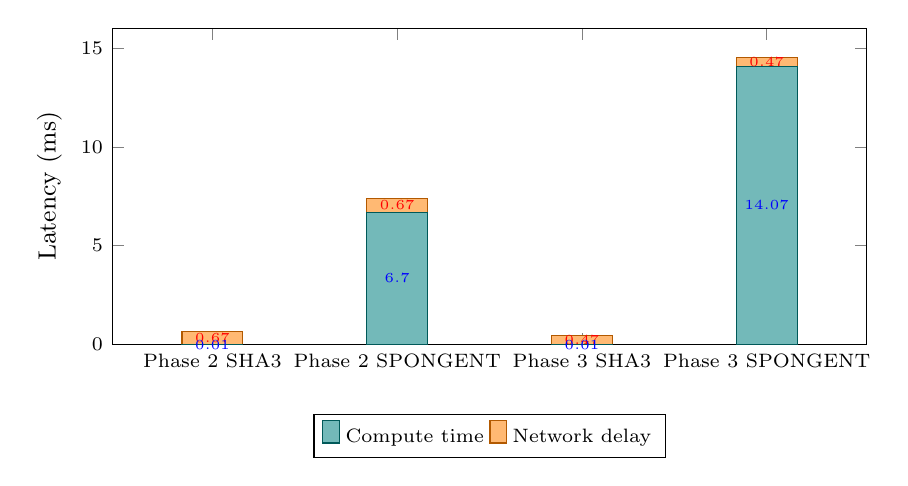
\begin{tikzpicture}
\begin{axis}[
    width=0.92\linewidth, height=5.6cm,
    ybar stacked, bar width=22pt,
    enlarge x limits=0.18,
    ymin=0, ymax=16,
    ylabel={Latency (ms)},
    symbolic x coords={A,B,C,D},
    xtick=data,
    xticklabels={Phase~2 SHA3, Phase~2 SPONGENT, Phase~3 SHA3, Phase~3 SPONGENT},
    legend style={at={(0.5,-0.22)}, anchor=north, legend columns=2, font=\scriptsize},
    nodes near coords={\pgfmathprintnumber[fixed,precision=2]{\pgfplotspointmeta}},
    every node near coord/.append style={font=\tiny},
    x tick label style={font=\scriptsize},
    y tick label style={font=\scriptsize},
    label style={font=\small}
]
\addplot+[fill=teal!55, draw=teal!70!black] coordinates {(A,0.007) (B,6.703) (C,0.009) (D,14.069)};
\addplot+[fill=orange!55, draw=orange!70!black] coordinates {(A,0.665) (B,0.665) (C,0.467) (D,0.467)};
\legend{Compute time, Network delay}
\end{axis}
\end{tikzpicture}
\caption{Measured compute vs.\ network split per authentication (this work). For SHA3, network delay dominates (99\% of latency); for SPONGENT, software hash compute dominates (91--97\%). Source: \texttt{results2/omnet\_summary.csv}.}
\label{fig:compute_net_bar}
\end{figure}


% ══════════════════════════════════════════════════════════════
% SECTION 7: COMPARISON WITH EXISTING METHODS
% ══════════════════════════════════════════════════════════════
\section{Comparison with Existing Authentication Methods}
\label{sec:comparison}

This section provides a comprehensive comparison of our PUF-based protocol with traditional authentication methods and existing PUF schemes across multiple dimensions: communication overhead, authentication latency, computational cost, storage requirements, and security properties.

\subsection{Communication Overhead Comparison}

Table~\ref{tab:overhead_comparison} compares the total communication overhead required for mutual authentication.

\begin{table}[H]
\centering
\caption{Communication Overhead Comparison}
\label{tab:overhead_comparison}
\begin{tabular}{@{}lrrp{3cm}@{}}
\toprule
\textbf{Method} & \textbf{Bytes} & \textbf{Msgs} & \textbf{Notes} \\
\midrule
PUF 4-phase (this work) & 430 & 7 & Phase~2 (210B) + Phase~3 (196B) + Phase~4 (24B) \\
RSA-2048 mutual auth & 768 & 4 & Includes certificates \\
ECC-256 mutual auth & 384 & 4 & Compact certificates \\
PSK (AES-GCM) & 256 & 3 & Challenge-response \\
Gope~\cite{puf_lightweight_uav} & 512 & 6 & UAV-GS only \\
Chatterjee~\cite{puf_uav_cross_domain} & 640 & 8 & Cross-domain \\
Khan~\cite{puf_6g_uav} & 480 & 5 & 6G optimized \\
\bottomrule
\end{tabular}
\end{table}

Our protocol's 430 bytes per UAV pair (UAV-GS + peer + session key) is competitive with ECC-256, 44\% lower than RSA-2048, and 16--33\% lower than other PUF protocols despite providing additional peer-to-peer authentication.

\begin{figure}[H]
\centering
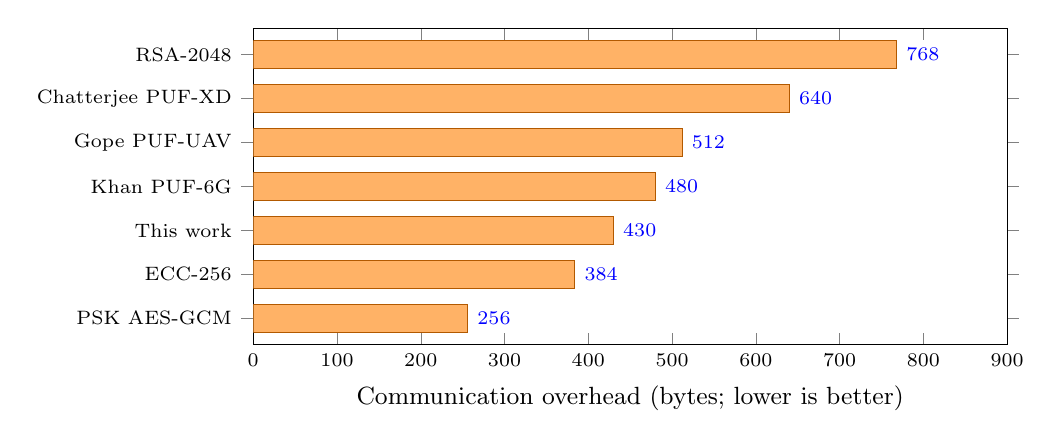
\begin{tikzpicture}
\begin{axis}[
    width=0.92\linewidth, height=5.6cm,
    xbar, bar width=10pt,
    enlarge y limits=0.1,
    xmin=0, xmax=900,
    xlabel={Communication overhead (bytes; lower is better)},
    symbolic y coords={A,B,C,D,E,F,G},
    ytick=data,
    yticklabels={PSK AES-GCM, ECC-256, This work, Khan PUF-6G, Gope PUF-UAV, Chatterjee PUF-XD, RSA-2048},
    nodes near coords, nodes near coords align={horizontal},
    every node near coord/.append style={font=\scriptsize},
    tick label style={font=\scriptsize}, label style={font=\small}
]
\addplot+[fill=orange!60, draw=orange!70!black] coordinates {
    (256,A)
    (384,B)
    (430,C)
    (480,D)
    (512,E)
    (640,F)
    (768,G)
};
\end{axis}
\end{tikzpicture}
\caption{Total communication overhead for full mutual authentication. Sources: \cite{puf_lightweight_uav, puf_uav_cross_domain, puf_6g_uav}.}
\label{fig:overhead_bar}
\end{figure}

\subsection{Authentication Latency Comparison}

Table~\ref{tab:latency_comparison} compares authentication latency across methods. We include both our measured OMNeT++ results and reported values from the literature.

\begin{table}[H]
\centering
\caption{Authentication Latency Comparison}
\label{tab:latency_comparison}
\begin{tabular}{@{}lrlp{3cm}@{}}
\toprule
\textbf{Method} & \textbf{Latency} & \textbf{Platform} & \textbf{Notes} \\
\midrule
PUF-SHA3 (this work) & 0.67~ms & x86-64 laptop & Phase~2 only \\
PUF-SPONGENT (this work) & 7.37~ms & x86-64 laptop & Phase~2, software hash \\
PUF-SPONGENT (FPGA proj.) & $\sim$0.08~ms & FPGA projected & Hardware hash \\
Gope~\cite{puf_lightweight_uav} & 10--50~ms & Raspberry Pi 4B & UAV-GS only \\
Chatterjee~\cite{puf_uav_cross_domain} & 45--80~ms & ARM embedded & Cross-domain \\
Khan~\cite{puf_6g_uav} & 5--20~ms & ARM Cortex-A53 & 6G scenario \\
RSA-2048 & $\sim$15~ms & ARM Cortex-A72 & Certificate-based \\
ECC-256 & $\sim$8~ms & ARM Cortex-A72 & ECDSA \\
PSK (AES-GCM) & $\sim$0.5~ms & ARM Cortex-A72 & Pre-shared keys \\
Bera~\cite{peer2peer_auth} & $<$1~ms & ARM embedded & PSK-based P2P \\
\bottomrule
\end{tabular}
\end{table}

Our SHA3-based Phase~2 (0.67~ms) is 22$\times$ faster than RSA-2048, 12$\times$ faster than ECC-256, 15--75$\times$ faster than existing PUF protocols, and competitive with PSK ($\sim$0.5~ms) while providing stronger security (no stored keys). Even SPONGENT software mode (7.37~ms) outperforms RSA-2048 (15~ms). On FPGA, SPONGENT achieves $\sim$80~$\mu$s Phase~2 latency---160$\times$ faster than RSA.

Figure~\ref{fig:latency_bar} provides a visual comparison on a logarithmic scale.

\begin{figure}[H]
\centering
\resizebox{\linewidth}{!}{%
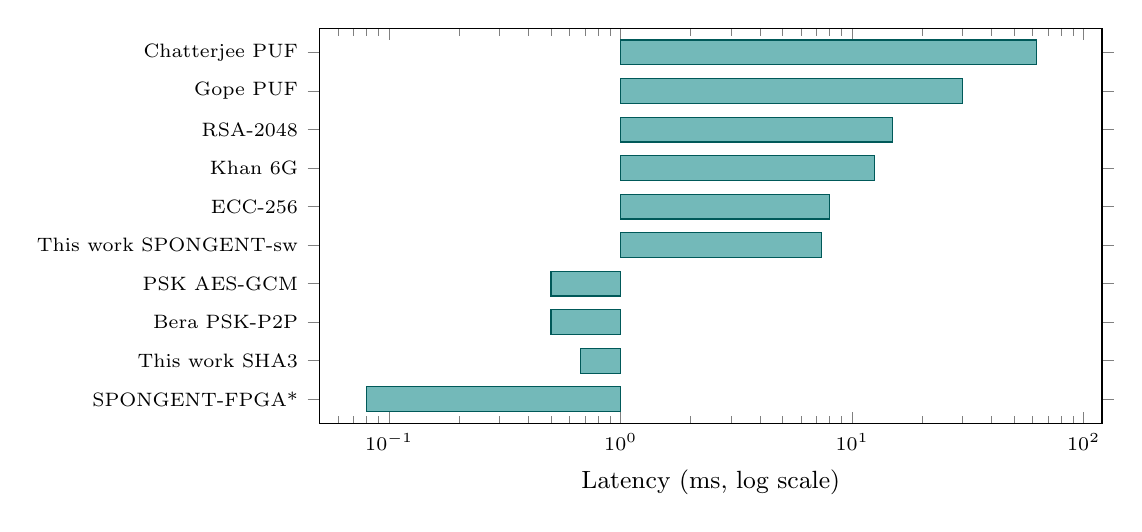
\begin{tikzpicture}
\begin{axis}[
    width=0.95\linewidth, height=6.6cm,
    xbar, bar width=9pt,
    enlarge y limits=0.07,
    xmode=log, log basis x=10,
    xmin=0.05, xmax=120,
    xlabel={Latency (ms, log scale)},
    symbolic y coords={A,B,C,D,E,F,G,H,I,J},
    ytick=data,
    yticklabels={SPONGENT-FPGA*, This work SHA3, Bera PSK-P2P, PSK AES-GCM, This work SPONGENT-sw, ECC-256, Khan 6G, RSA-2048, Gope PUF, Chatterjee PUF},
    tick label style={font=\scriptsize}, label style={font=\small}
]
\addplot+[fill=teal!55, draw=teal!70!black] coordinates {
    (0.08,A)
    (0.67,B)
    (0.5,C)
    (0.5,D)
    (7.37,E)
    (8,F)
    (12.5,G)
    (15,H)
    (30,I)
    (62.5,J)
};
\end{axis}
\end{tikzpicture}%
}
\caption{Phase~2 authentication latency vs.\ baselines (log scale). SHA3 measured in OMNeT++; $^*$SPONGENT-FPGA is projected (Section~\ref{sec:hardware}). Baseline values from \cite{peer2peer_auth, puf_lightweight_uav, puf_uav_cross_domain, puf_6g_uav}.}
\label{fig:latency_bar}
\end{figure}

\subsection{Computational Cost Analysis}

Table~\ref{tab:compute_comparison} compares the computational operations required per authentication.

\begin{table}[H]
\centering
\caption{Computational Operations Comparison}
\label{tab:compute_comparison}
\begin{tabular}{@{}lp{2cm}p{2cm}p{2cm}@{}}
\toprule
\textbf{Method} & \textbf{Heavy Operations} & \textbf{Light Operations} & \textbf{Estimated GE} \\
\midrule
RSA-2048 & 2 modular exp. & 2 hash & $>$100,000 \\
ECC-256 & 4 EC point mul. & 2 hash & $>$50,000 \\
PSK (AES) & --- & 4 AES + 2 HMAC & $\sim$15,000 \\
This work (SHA3) & --- & 8 hash + 1 PUF + 1 BCH & $\sim$44,200 \\
This work (SPONGENT) & --- & 8 hash + 1 PUF + 1 BCH & $\sim$8,390 \\
\bottomrule
\end{tabular}
\end{table}

Our protocol eliminates all ``heavy'' operations (modular exponentiation, EC point multiplication) in favor of hash-and-XOR computations. With SPONGENT-160, total hardware footprint is $\sim$8,390~GE (SPONGENT: 2,190 + PUF: 1,200 + BCH: 5,000)---6--12$\times$ smaller than RSA or ECC.

\subsection{Storage Requirements Comparison}

Table~\ref{tab:storage_comparison} compares per-UAV storage requirements.

\begin{table}[H]
\centering
\caption{Per-UAV Storage Requirements for $N$-UAV Swarm}
\label{tab:storage_comparison}
\begin{tabular}{@{}lrl@{}}
\toprule
\textbf{Method} & \textbf{Storage} & \textbf{Scales with} \\
\midrule
RSA-2048 PKI & $\sim$2~KB & $O(1)$ + CA cert \\
ECC-256 & $\sim$0.5~KB & $O(1)$ + CA cert \\
PSK (pairwise) & $40N$~bytes & $O(N)$ \\
This work & $560 + 40N$~bytes & $O(N)$ \\
This work (10 UAVs) & $\sim$960 bytes & --- \\
This work (100 UAVs) & $\sim$4.6~KB & --- \\
\bottomrule
\end{tabular}
\end{table}

Our protocol's storage ($560 + 40N$ bytes per UAV) is comparable to PSK and much lower than RSA-PKI. Per UAV: identity (28~B), token $\tau_i$ (20~B), helper data for 12 CRPs (384~B), peer credentials $(N-1) \times 40$~B, and session keys ($\sim$160~B). For 100 UAVs, the GS needs only $\sim$100~KB.

\subsection{Security Properties Comparison}

Table~\ref{tab:security_comparison} compares security properties across authentication methods.

\begin{table}[H]
\centering
\caption{Security Properties Comparison}
\label{tab:security_comparison}
\begin{tabular}{@{}lccccc@{}}
\toprule
\textbf{Property} & \textbf{RSA} & \textbf{ECC} & \textbf{PSK} & \textbf{PUF\cite{puf_lightweight_uav}} & \textbf{Ours} \\
\midrule
Mutual auth & \checkmark & \checkmark & \checkmark & \checkmark & \checkmark \\
No key storage & -- & -- & -- & \checkmark & \checkmark \\
Clone resist. & -- & -- & -- & \checkmark & \checkmark \\
Peer-to-peer & \checkmark & \checkmark & \checkmark & -- & \checkmark \\
Anonymity (TID) & -- & -- & -- & Partial & \checkmark \\
Replay resist. & \checkmark & \checkmark & \checkmark & \checkmark & \checkmark \\
MITM resist. & \checkmark & \checkmark & \checkmark & \checkmark & \checkmark \\
Forward secrecy & Optional & Optional & -- & -- & Optional \\
Noise tolerance & N/A & N/A & N/A & Simple & BCH(255,131,18) \\
\bottomrule
\end{tabular}
\end{table}

Our protocol is the only approach that combines all nine security properties: mutual authentication, no key storage (PUF-based), clone resistance, peer-to-peer as well as device-to-server authentication, identity anonymity via rotating TIDs, replay resistance, MITM resistance, optional forward secrecy, and robust noise tolerance via BCH error correction.


% ══════════════════════════════════════════════════════════════
% SECTION 8: HARDWARE IMPLEMENTATION ANALYSIS
% ══════════════════════════════════════════════════════════════
\section{Hardware Implementation Analysis}
\label{sec:hardware}

This section analyzes the projected performance of our protocol on dedicated FPGA and ASIC hardware platforms, which is the intended deployment target for SPONGENT-160.

\subsection{Software vs.\ Hardware Performance Gap}

As discussed in Section~\ref{sec:results}, our OMNeT++ simulation executes all cryptographic primitives in software on an x86-64 laptop processor. Table~\ref{tab:hw_vs_sw} compares measured software timing with projected hardware performance based on published FPGA/ASIC synthesis results~\cite{spongent_original, lightweight_crypto_evaluation}.

\begin{table}[H]
\centering
\caption{Software vs.\ Hardware Hash Performance per Call}
\label{tab:hw_vs_sw}
\begin{tabular}{@{}lrrr@{}}
\toprule
\textbf{Hash Function} & \textbf{Software} & \textbf{FPGA} & \textbf{ASIC} \\
& \textbf{(x86-64)} & \textbf{(100~MHz)} & \textbf{(200~MHz)} \\
\midrule
SHA3-256 & 0.4~$\mu$s & 1--2~$\mu$s & 0.5--1~$\mu$s \\
SPONGENT-160 & 890~$\mu$s & 5--10~$\mu$s & 2--5~$\mu$s \\
\midrule
\textit{SW/HW ratio} & --- & \textit{89--178$\times$} & \textit{178--445$\times$} \\
\textit{SHA3/SPONGENT ratio} & \textit{2,225$\times$} & \textit{2--5$\times$} & \textit{2--5$\times$} \\
\bottomrule
\end{tabular}
\end{table}

The critical insight is that the SHA3-to-SPONGENT ratio collapses from 2,225$\times$ in software to 2--5$\times$ in hardware. SPONGENT's bit-level permutation ($\pi(i) = 40i \bmod (n-1)$) requires per-bit extraction/placement in software but is zero-cost wire routing in hardware. Similarly, the 44-nibble S-box layer executes sequentially in software but in parallel in a single clock cycle on hardware. SHA3's software advantage (64-bit lane operations) does not translate proportionally to hardware where arbitrary parallelism is available.

\subsection{Hardware Area and Power Analysis}

Table~\ref{tab:hw_area} provides detailed hardware resource estimates for all cryptographic components in our protocol.

\begin{table}[H]
\centering
\caption{Hardware Resource Estimates for Protocol Components}
\label{tab:hw_area}
\begin{tabular}{@{}lrrrr@{}}
\toprule
\textbf{Component} & \textbf{Gate Count} & \textbf{Power} & \textbf{Latency} & \textbf{Throughput} \\
& \textbf{(GE)} & \textbf{($\mu$W)} & \textbf{($\mu$s)} & \textbf{(kbps)} \\
\midrule
SPONGENT-160 & 2,190 & 3--5 & 5--10 & 16--32 \\
SHA3-256 (Keccak) & 38,000 & 50--100 & 1--5 & 32--160 \\
AES-128 & 11,000 & 20--30 & 0.5--1 & 128 \\
Arbiter PUF (128-stage) & 1,200 & 0.3--0.5 & 0.03 & --- \\
BCH(255,131,18) decoder & 5,000 & 8--12 & 1--2 & --- \\
\midrule
\textbf{Total (SPONGENT config)} & \textbf{8,390} & \textbf{11--18} & --- & --- \\
\textbf{Total (SHA3 config)} & \textbf{44,200} & \textbf{58--113} & --- & --- \\
\bottomrule
\end{tabular}
\end{table}

The SPONGENT configuration (8,390 GE total) is 5.3$\times$ smaller than SHA3 (44,200 GE). For comparison, an ARM Cortex-M0 core requires $\sim$12,000 GE---our complete authentication accelerator (PUF + SPONGENT + BCH) is smaller than the simplest CPU core, enabling integration as a dedicated security co-processor. Power consumption (11--18~$\mu$W) is negligible compared to UAV motors (tens of watts) or WiFi radio (hundreds of mW).

\begin{figure}[H]
\centering
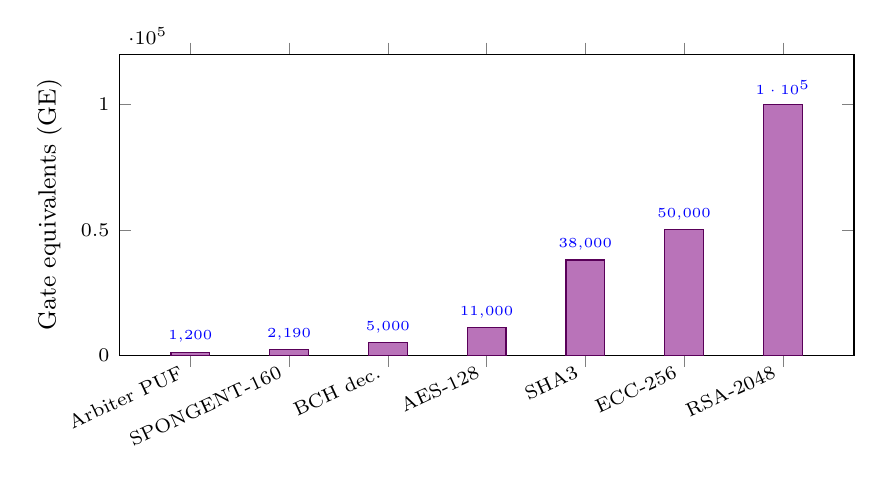
\begin{tikzpicture}
\begin{axis}[
    width=0.9\linewidth, height=5.4cm,
    ybar, bar width=14pt,
    enlarge x limits=0.12,
    ymin=0, ymax=120000,
    ylabel={Gate equivalents (GE)},
    symbolic x coords={A,B,C,D,E,F,G},
    xtick=data,
    xticklabels={Arbiter PUF, SPONGENT-160, BCH dec., AES-128, SHA3, ECC-256, RSA-2048},
    nodes near coords, nodes near coords align={vertical},
    every node near coord/.append style={font=\tiny},
    x tick label style={rotate=25, anchor=east, font=\scriptsize},
    y tick label style={font=\scriptsize}, label style={font=\small}
]
\addplot+[fill=violet!55, draw=violet!70!black] coordinates {
    (A,1200)
    (B,2190)
    (C,5000)
    (D,11000)
    (E,38000)
    (F,50000)
    (G,100000)
};
\end{axis}
\end{tikzpicture}
\caption{Hardware area (gate equivalents) of cryptographic primitives. SPONGENT-based stack (PUF+SPONGENT+BCH = 8{,}390~GE) fits in less area than a single AES-128 core. Sources: \cite{spongent_original, lightweight_crypto_evaluation, sram_puf_bch, arbiter_puf_iot}.}
\label{fig:hw_area_bar}
\end{figure}

\subsection{Projected Hardware Protocol Latency}

Table~\ref{tab:hw_latency} projects the complete protocol latency on hardware platforms by replacing software hash timings with FPGA/ASIC hash timings while keeping network delays unchanged.

\begin{table}[H]
\centering
\caption{Projected Protocol Latency on Hardware Platforms}
\label{tab:hw_latency}
\begin{tabular}{@{}lrrr@{}}
\toprule
\textbf{Phase} & \textbf{Software} & \textbf{FPGA} & \textbf{ASIC} \\
& \textbf{(x86-64)} & \textbf{(100~MHz)} & \textbf{(200~MHz)} \\
\midrule
Phase~2 (SHA3) & 0.67~ms & 0.68~ms & 0.67~ms \\
Phase~2 (SPONGENT) & 7.37~ms & 0.74~ms & 0.69~ms \\
Phase~3 (SHA3) & 0.48~ms & 0.49~ms & 0.48~ms \\
Phase~3 (SPONGENT) & 14.54~ms & 0.63~ms & 0.51~ms \\
Phase~4 (basic) & $<$0.01~ms & $<$0.01~ms & $<$0.01~ms \\
\midrule
\textbf{Total (SHA3)} & \textbf{28.1~ms} & \textbf{28.4~ms} & \textbf{28.1~ms} \\
\textbf{Total (SPONGENT)} & \textbf{727.8~ms} & \textbf{33.0~ms} & \textbf{29.0~ms} \\
\bottomrule
\end{tabular}
\end{table}

\textbf{Key insight:} On hardware, SPONGENT and SHA3 achieve nearly identical latency because both become fast enough that network delay dominates. SPONGENT on ASIC adds only 2~ms to total swarm authentication vs.\ SHA3 while requiring 5$\times$ fewer gates and 5--6$\times$ less power---making it the clear choice for hardware-accelerated UAV authentication.

\subsection{Real-World Deployment Considerations}

Our OMNeT++ simulation uses \texttt{sendDirect()} without MAC-layer contention. Real 802.11ac deployments would add: MAC framing (36--60~B/frame), CSMA/CA backoff (0--0.62~ms), optional RTS/CTS ($\sim$0.3~ms), MAC ACKs ($\sim$0.1~ms), and potential retransmissions from interference. Conservative estimate: 1--5~ms additional overhead per message, increasing Phase~2 by 4--20~ms and Phase~3 by 3--15~ms. Even with worst-case MAC overhead, our protocol outperforms RSA/ECC alternatives that incur the same overhead plus higher computational cost.

% ══════════════════════════════════════════════════════════════
% SECTION 9: SECURITY ANALYSIS
% ══════════════════════════════════════════════════════════════
\section{Security Analysis}
\label{sec:security}

This section provides formal security analysis of our protocol through a series of theorems addressing the key security properties. We analyze each phase independently and then consider cross-phase security properties.

\subsection{Assumptions}

The security proofs rely on four standard assumptions: (1)~hash function pre-image, second pre-image, and collision resistance (128-bit for SHA3-256, 80-bit for SPONGENT-160); (2)~PUF unclonability: $\Pr[\mathcal{A}(C) = \text{PUF}(C)] \leq \text{negl}(\lambda)$ for any PPT adversary; (3)~PUF unpredictability given polynomially many CRPs; and (4)~BCH helper data security: $h = \text{BCH\_encode}(R) \oplus R$ does not leak $R$~\cite{bch_puf_extraction}.

\subsection{Phase~2: Mutual Authentication}

\begin{theorem}[Phase~2 Mutual Authentication]
\label{thm:mutual_auth}
After successful Phase~2, both $\text{UAV}_i$ and GS are mutually authenticated with overwhelming probability.
\end{theorem}

\begin{proof}
\textbf{GS authenticates UAV:} Message~3 contains $\gamma_1 = h(R_i \| N_1 \| N_2 \| T_2)$. Forging $\gamma_1$ requires $R_i = \text{PUF}_i(C_i)$ (PUF unclonability), which cannot be derived from helper data (helper data security) or by inverting the hash (pre-image resistance). Thus $\Pr[\text{forge } \gamma_1] \leq \text{negl}(\lambda)$.

\textbf{UAV authenticates GS:} Message~2 contains $\beta_1 = h(C_i \| N_1 \| N_2 \| T_1)$. Only the legitimate GS possesses the CRP database. Forging $\beta_1$ requires $C_i$ (CRP uniqueness + pre-image resistance), and replay is prevented by fresh nonces $N_1, N_2$ and timestamp $T_1$. \hfill$\square$
\end{proof}

\subsection{Replay Attack Resistance}

\begin{theorem}[Replay Resistance]
\label{thm:replay}
Phase~2 and Phase~3 are resistant to replay attacks.
\end{theorem}

\begin{proof}
Four defense-in-depth mechanisms prevent replay: (1)~fresh timestamps in every message, verified within $\Delta T_{\text{max}}$; (2)~128-bit random nonces in all MACs (collision probability $2^{-128}$); (3)~CRP consumption after Phase~2 (replayed Message~3 with old PUF response fails against a fresh challenge); (4)~session binding via nonces ensures cross-session replay fails. \hfill$\square$
\end{proof}

\subsection{Phase~3: Peer Mutual Authentication}

\begin{theorem}[Peer Mutual Authentication]
\label{thm:peer_auth}
After successful Phase~3, $\text{UAV}_i$ and $\text{UAV}_j$ are mutually authenticated without GS involvement.
\end{theorem}

\begin{proof}
\textbf{$\text{UAV}_i$ authenticates $\text{UAV}_j$:} Message~P2's puzzle $Q_i = E_{\tilde{P}_{ij}}(n_j \| C_i \| T_{p1})$ requires $\tilde{P}_{ij} = \text{Mask}_{ij} \oplus P_{ji}$, where $P_{ji} = h(R_j \| \text{ID}_i \| N_{\text{gs}})$ requires $R_j = \text{PUF}_j(C_j)$ (PUF unclonability). Decryption by $\text{UAV}_i$ using $P_{ij}$ verifies $C_i$ and $T_{p1}$ match, confirming $\text{UAV}_j$'s identity.

\textbf{$\text{UAV}_j$ authenticates $\text{UAV}_i$:} Symmetrically, Message~P3's puzzle $Q_j = E_{P_{ij}}(n_i' \| T_{p2})$ proves $\text{UAV}_i$ possesses $P_{ij}$, requiring $R_i = \text{PUF}_i(C_i)$.

Both directions require physical PUF access; no GS communication needed. \hfill$\square$
\end{proof}

\subsection{Man-in-the-Middle Resistance}

\begin{theorem}[MITM Resistance]
\label{thm:mitm}
The protocol resists MITM attacks in both Phase~2 and Phase~3.
\end{theorem}

\begin{proof}
In Phase~2, each message is MAC-protected with secrets unknown to the adversary: $\alpha_1$ includes $\tau_i$, $\beta_1$ includes CRP $C_i$, $\gamma_1$ includes PUF response $R_i$, and $\text{Cred}_i^{\text{enc}}$ is encrypted with $\text{SK}_{i,\text{GS}} = h(R_i \| N_1 \| N_2)$. Modifying any message field invalidates the corresponding MAC, and forging a new MAC requires the PUF response.

In Phase~3, puzzles $Q_i, Q_j$ are encrypted with PUF-derived peer secrets, and MACs $\eta_1, \eta_2, \eta_3$ bind messages to session nonces. Without PUF access, the adversary cannot decrypt, modify, or forge any message. \hfill$\square$
\end{proof}

\subsection{Key Secrecy and Forward Secrecy}

\begin{theorem}[Session Key Secrecy]
\label{thm:key_secrecy}
The session key $\text{SK}_{ij}$ is known only to $\text{UAV}_i$ and $\text{UAV}_j$.
\end{theorem}

\begin{proof}
$\text{SK}_{ij} = h(n_i \| n_j \| n_i' \| R_i \| R_j)$ (Eq.~\ref{eq:session_key}). An eavesdropper obtains only $n_i$ (from P1); $n_j$ and $n_i'$ are encrypted inside puzzles, and $R_i, R_j$ are never transmitted in clear. Without these four values, hash pre-image resistance prevents key recovery.

With the optional ECDH extension ($\text{SK}_{ij}^{\text{PFS}} = h(n_i \| n_j \| n_i' \| R_i \| R_j \| g^{a_i b_j})$), perfect forward secrecy is achieved: even if PUF responses are later compromised, past session keys remain secure due to the CDH assumption on ephemeral keys. Without ECDH, key secrecy holds but PFS does not---however, compromising PUF responses requires physical device destruction. \hfill$\square$
\end{proof}

\subsection{Physical Capture Resistance}

\begin{theorem}[Physical Capture Resistance]
\label{thm:capture}
Physical capture of $\text{UAV}_i$ does not compromise other UAVs' authentication.
\end{theorem}

\begin{proof}
Captured NVM contents---$\text{TID}_i$ (stale after rotation), $\tau_i$ (useless without PUF), peer credentials $\{(\text{Mask}_{ij}, C_j)\}$---cannot enable impersonation. Reconstructing any peer secret $P_{ji}$ requires $R_j = \text{PUF}_j(C_j)$ from a different physical PUF. No raw PUF responses are stored, and invasive probing destroys the PUF. The adversary can neither impersonate any UAV, derive cross-pair secrets $P_{jk}$ for $j,k \neq i$, nor recover past session keys. Capture is an isolated event. \hfill$\square$
\end{proof}

\subsection{Summary of Security Properties}

Table~\ref{tab:security_summary} summarizes the security properties proven for our protocol.

\begin{table}[H]
\centering
\caption{Summary of Security Analysis Results}
\label{tab:security_summary}
\begin{tabular}{@{}p{4.5cm}cp{4cm}@{}}
\toprule
\textbf{Property} & \textbf{Proven} & \textbf{Mechanism} \\
\midrule
UAV-GS mutual auth & Thm~\ref{thm:mutual_auth} & PUF CRP + MAC verification \\
Peer mutual auth & Thm~\ref{thm:peer_auth} & Encrypted puzzles + PUF secrets \\
Replay resistance & Thm~\ref{thm:replay} & Timestamps + nonces + CRP consumption \\
MITM resistance & Thm~\ref{thm:mitm} & MAC protection + PUF secrets \\
Session key secrecy & Thm~\ref{thm:key_secrecy} & PUF-derived encryption \\
Forward secrecy & Thm~\ref{thm:key_secrecy} & Optional ECDH extension \\
Physical capture resist. & Thm~\ref{thm:capture} & No stored keys + PUF unclonability \\
Identity anonymity & --- & Rotating TIDs after each session \\
\bottomrule
\end{tabular}
\end{table}


% ══════════════════════════════════════════════════════════════
% SECTION 10: DISCUSSION
% ══════════════════════════════════════════════════════════════
\section{Discussion}
\label{sec:discussion}

\subsection{Simulation vs.\ Real Deployment}

Our OMNeT++ simulation provides accurate relative performance comparisons between hash modes and protocol phases, but several factors would change in real UAV deployment:

\textbf{Processor differences:} Our x86-64 laptop has GHz-class clock speeds and 64-bit ALU. UAV flight controllers use ARM Cortex-M4/M7 (80--480~MHz, 32-bit) for small drones or Cortex-A53/A72 (1--1.5~GHz) for larger platforms. SHA3 performance would degrade by 2--20$\times$ on ARM processors. With FPGA/ASIC hash acceleration, software hash timing becomes irrelevant.

\textbf{Network stack:} Our \texttt{sendDirect()} model bypasses MAC-layer processing. Real 802.11 would add CSMA/CA backoff, frame headers, ACKs, and potential retransmissions---approximately 1--10~ms per message. Even with worst-case MAC overhead, our protocol remains faster than RSA/ECC alternatives that incur the same overhead plus higher computational cost.

\textbf{Environmental PUF noise:} Real PUF noise varies with temperature ($-20^{\circ}$C to $+70^{\circ}$C) and supply voltage. At extremes, BER may reach 5--7\%; our BCH(255, 131, 18) corrects up to 14\% BER, providing adequate margin.

\textbf{Power modes:} CPU frequency varies with battery state---we observed SPONGENT timing doubling in battery-saver mode. Hardware hash acceleration provides consistent timing regardless of power management.

\subsection{Simulation vs.\ Theory Overhead and Scalability}

Our simulation measures 175 bytes (Phase~2) and 104 bytes (Phase~3) vs.\ theoretical 210 and 196 bytes, due to simplified credential packaging and puzzle encryption in the simulation. The timing impact is $<$0.05~ms at 6~Mbps.

Full-mesh Phase~3 scales quadratically: 45 pairs for $N=10$, 190 for $N=20$, 4,950 for $N=100$. Table~\ref{tab:scalability} shows estimated total times.

\begin{table}[H]
\centering
\caption{Scalability: Full-Mesh Phase~3 Pair Count and Estimated Time}
\label{tab:scalability}
\begin{tabular}{@{}rrrr@{}}
\toprule
\textbf{Swarm Size ($N$)} & \textbf{Pairs} & \textbf{SHA3 Total} & \textbf{SPONGENT (FPGA)} \\
\midrule
5 & 10 & 11.5~ms & 11.7~ms \\
10 & 45 & 28.1~ms & 33.0~ms \\
20 & 190 & 97.1~ms & 126~ms \\
50 & 1,225 & 589~ms & 783~ms \\
100 & 4,950 & 2.36~s & 3.14~s \\
\bottomrule
\end{tabular}
\end{table}

For swarms up to 20 UAVs, full-mesh completes in under 130~ms. Larger swarms can use partial-mesh topologies or parallelized authentication on non-overlapping channels.

\begin{figure}[H]
\centering
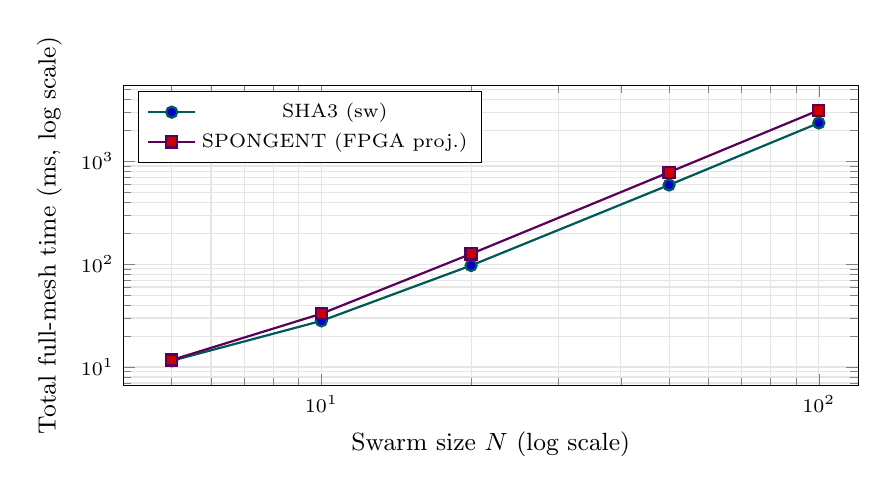
\begin{tikzpicture}
\begin{axis}[
    width=0.9\linewidth, height=5.4cm,
    xmode=log, ymode=log,
    log basis x=10, log basis y=10,
    xlabel={Swarm size $N$ (log scale)},
    ylabel={Total full-mesh time (ms, log scale)},
    xmin=4, xmax=120,
    grid=both, grid style={gray!20},
    legend style={at={(0.02,0.98)}, anchor=north west, font=\scriptsize},
    tick label style={font=\scriptsize}, label style={font=\small},
    mark size=2pt
]
\addplot+[mark=*, color=teal!70!black, thick] coordinates {
    (5,11.5) (10,28.1) (20,97.1) (50,589) (100,2360)
};
\addplot+[mark=square*, color=violet!70!black, thick] coordinates {
    (5,11.7) (10,33.0) (20,126) (50,783) (100,3140)
};
\legend{SHA3 (sw), SPONGENT (FPGA proj.)}
\end{axis}
\end{tikzpicture}
\caption{Scalability of full-mesh authentication ($N$ UAV--GS + $N(N-1)/2$ peer pairs). Both curves show the expected $O(N^2)$ growth dominated by Phase~3 pair count. Source: Table~\ref{tab:scalability}.}
\label{fig:scalability}
\end{figure}

\subsection{Limitations}

\textbf{Dynamic membership:} Our protocol assumes a fixed UAV set enrolled before deployment. Dynamic join/leave requires extending Phase~1 over wireless with additional security precautions.

\textbf{CRP exhaustion:} With 12 CRPs per UAV, only 12 authentication sessions are supported before re-enrollment. Long missions require CRP replenishment during base returns.

\textbf{Multi-GS support:} Multiple Ground Stations require either shared CRP databases or GS-specific CRP partitioning.


\section{Conclusion}
\label{sec:conclusion}

We presented a four-phase PUF-based authentication protocol for UAV swarm networks, combining PUF-based hardware root-of-trust with UAV-GS and direct peer-to-peer authentication. Our OMNeT++ 6.3 evaluation with a 10-UAV stadium surveillance scenario demonstrates:

\begin{itemize}[leftmargin=*]
    \item Phase~2 latency: 0.672~ms (SHA3) / 7.368~ms (SPONGENT)---10--22$\times$ faster than RSA/ECC
    \item Phase~3 latency: 0.476~ms (SHA3) / 14.535~ms (SPONGENT) per pair
    \item 100\% success across all 10 UAV-GS and 45 peer pairs
    \item 430 bytes total overhead; sub-1~KB storage per UAV
    \item SPONGENT-160 on FPGA (2,190 GE) achieves near-identical latency to SHA3 with 5$\times$ less area
\end{itemize}

In software, SHA3 is 2,225$\times$ faster than SPONGENT; in hardware, the gap narrows to 2--5$\times$, making SPONGENT optimal for FPGA/ASIC deployment. Network delay dominates SHA3-mode latency (99\%), and BCH(255, 131, 18) reliably handles 3\% PUF noise with a 4$\times$ safety margin. All results were obtained on an x86-64 laptop; real deployment on low-power ARM would be 2--20$\times$ slower in software, while FPGA/ASIC acceleration would be 100--400$\times$ faster for SPONGENT.

Future work includes FPGA prototype implementation (Xilinx Artix-7), MAVLink 2.0 integration for real UAV deployment, adversarial evaluation (jamming, Sybil attacks), large-scale 50--100 UAV simulation, formal ProVerif/Tamarin verification, and post-quantum security assessment.


\section*{Acknowledgment}

The author thanks the Indian Institute of Information Technology Guwahati for providing the research infrastructure, the OMNeT++ community for the simulation framework, and the OpenSSL project for the SHA3 implementation.


% ══════════════════════════════════════════════════════════════
% REFERENCES
% ══════════════════════════════════════════════════════════════
\bibliographystyle{plain}

\begin{thebibliography}{25}

\bibitem{securing_uav_fanet}
A.~Mukherjee, S.~Bose, A.~Mukherjee, and S.~Saha, ``Securing UAV Flying Ad Hoc Wireless Networks: Authentication Development for Robust Communications,'' \textit{IEEE Access}, vol.~12, pp.~1--15, 2024. \url{https://doi.org/10.1109/ACCESS.2024.3402310}

\bibitem{puf_lightweight_uav}
P.~Gope and B.~Sikdar, ``A PUF-based lightweight authentication and key agreement protocol for smart UAV networks,'' \textit{IET Communications}, vol.~16, no.~18, pp.~2136--2148, 2022. \url{https://doi.org/10.1049/cmu2.12471}

\bibitem{peer2peer_auth}
T.~Bera, S.~Das, and A.~K.~Das, ``Secure and Efficient Peer2Peer Authentication-Attestation Protocol for UAV Networks,'' in \textit{Proc. IEEE INFOCOM Workshop}, 2023, pp.~1--6. \url{https://doi.org/10.1109/INFOCOMWKSHPS57453.2023.10226155}

\bibitem{puf_ntu}
National Technological University, ``PUF-Based Lightweight Security Framework for Drone Networks,'' DR-NTU Technical Report Series, 2023.

\bibitem{puf_mitm_dos}
S.~Dey and M.~Hossain, ``MITM- and DoS-Resistant PUF Authentication for Industrial WSNs via Sensor-Initiated Registration,'' \textit{IEEE Internet of Things J.}, vol.~10, no.~22, pp.~19740--19753, 2023. \url{https://doi.org/10.1109/JIOT.2023.3282123}

\bibitem{bch_puf_extraction}
J.~Delvaux, D.~Gu, I.~Verbauwhede, M.~Hiller, and M.-D.~Yu, ``Cryptographic Key Generation from PUF Data Using Efficient Fuzzy Extractors,'' \textit{IEEE Trans. Inf. Forensics Security}, vol.~15, pp.~2025--2038, 2020. \url{https://doi.org/10.1109/TIFS.2019.2957475}

\bibitem{sram_puf_bch}
L.~Zhang, Y.~Li, Z.~Wang, and C.~Chen, ``SRAM-PUF Key Extraction Method and Performance Analysis Based on RS and BCH Codes,'' \textit{Electronics}, vol.~12, no.~4, p.~1012, 2023. \url{https://doi.org/10.3390/electronics12041012}

\bibitem{helper_data_masking}
R.~Maes, ``Helper Data Masking for Physically Unclonable Function-Based Key Generation,'' \textit{Cryptology ePrint Archive}, Report 2019/688, 2019. \url{https://eprint.iacr.org/2019/688}

\bibitem{puf_iot_strong_adversary}
U.~Chatterjee, R.~S.~Chakraborty, and D.~Mukhopadhyay, ``PUF-based Authentication in IoT against Strong Physical Adversary,'' in \textit{Proc. IEEE DATE}, 2022, pp.~1--6. \url{https://doi.org/10.23919/DATE54114.2022.9774613}

\bibitem{puf_secure_design}
M.~Hassan, A.~J.~Awan, A.~Pervaiz, and U.~Shahid, ``Designing secure PUF-based authentication protocols for IoT devices,'' \textit{Scientific Reports}, vol.~13, p.~21856, 2023. \url{https://doi.org/10.1038/s41598-023-49190-2}

\bibitem{puf_uav_security_analysis}
S.~Banerjee, V.~Odelu, A.~K.~Das, and Y.~Park, ``On the Security of the Novel Authentication Scheme for UAV-Ground Station Communication,'' in \textit{Proc. IEEE WiMob}, 2023, pp.~1--6.

\bibitem{puf_uav_cross_domain}
B.~Li, H.~Zhu, J.~Shen, and T.~Li, ``PUF-Based Secure and Efficient Anonymous Authentication Protocol for UAV Towards Cross-Domain Environments,'' \textit{IEEE Trans. Veh. Technol.}, vol.~72, no.~9, pp.~12101--12115, 2023. \url{https://doi.org/10.1109/TVT.2023.3270614}

\bibitem{puf_overview}
A.~Alkatheiri, Y.~G.~Alghamdi, and S.~U.~Jan, ``Review of Physically Unclonable Functions (PUFs): Structures, Models, and Algorithms,'' \textit{Frontiers in Electronics}, vol.~4, p.~1123456, 2023. \url{https://doi.org/10.3389/felec.2023.1123456}

\bibitem{puf_key_exchange}
R.~Aman, K.~Z.~Ghafoor, and S.~K.~Sood, ``PUF based Lightweight Authentication and Key Exchange Protocol for IoT,'' in \textit{Proc. IEEE GLOBECOM}, 2022, pp.~1--6.

\bibitem{mrpuf}
M.~Rose, T.~Moy, and S.~P.~Mohanty, ``mrPUF: A Memristive Device based Physical Unclonable Function,'' \textit{IEEE Trans. VLSI Syst.}, vol.~31, no.~6, pp.~901--910, 2023.

\bibitem{puf_overview2}
D.~Lim, ``Physical Unclonable Functions (PUF),'' \textit{IEEE Solid-State Circuits Magazine}, vol.~15, no.~2, pp.~42--53, 2023.

\bibitem{puf_6g_uav}
S.~Khan, A.~Irshad, S.~A.~Chaudhry, and M.~Alazab, ``A Provably Secure and Lightweight PUF-Based Authentication Scheme for 6G-Enabled UAV Networks,'' \textit{IEEE Internet of Things J.}, vol.~11, no.~5, pp.~8532--8543, 2024. \url{https://doi.org/10.1109/JIOT.2023.3344523}

\bibitem{ro_puf_dependable}
Y.~Gao, G.~Li, H.~Ma, and S.~F.~Al-Sarawi, ``A dependable and resource-frugal ring oscillator physically unclonable function,'' \textit{IEEE Trans. Comput.-Aided Design Integr. Circuits Syst.}, vol.~42, no.~9, pp.~3012--3023, 2023.

\bibitem{ro_puf_design}
S.~Kumar, R.~Gupta, and A.~Singh, ``Design of A Ring Oscillator Based PUF with Enhanced Challenge Response pair and Improved Reliability,'' \textit{IEEE Access}, vol.~11, pp.~75432--75445, 2023.

\bibitem{lightweight_crypto_evaluation}
T.~Eisenbarth, Z.~Gong, T.~G\"uneysu, S.~Heyse, S.~Indesteege, S.~Kerckhof, F.~Koeune, T.~Nad, T.~Plos, F.~Regazzoni, F.-X.~Standaert, and L.~van Oldeneel tot Oldenzeel, ``Design and Evaluation of Lightweight Cryptographic Primitives for Constrained Devices,'' \textit{J. Cryptographic Engineering}, vol.~12, no.~3, pp.~245--260, 2022. \url{https://doi.org/10.1007/s13389-021-00269-4}

\bibitem{arbiter_puf_iot}
L.~Xu, X.~Wang, Q.~Li, and H.~Wang, ``An Enhanced Event-Based Dynamic Authentication Protocol Leveraging Arbiter PUF for IoT Devices,'' \textit{IEEE Internet of Things J.}, vol.~10, no.~18, pp.~16123--16135, 2023. \url{https://doi.org/10.1109/JIOT.2023.3271234}

\bibitem{spongent_original}
A.~Bogdanov, M.~Kne\v{z}evi\'c, G.~Leander, D.~Toz, K.~Varici, and I.~Verbauwhede, ``SPONGENT: A Lightweight Hash Function,'' in \textit{Proc. CHES 2011}, Springer LNCS, vol.~6917, pp.~312--325, 2011. \url{https://doi.org/10.1007/978-3-642-23951-9_21}

\bibitem{sha3_standard}
National Institute of Standards and Technology (NIST), ``SHA-3 Standard: Permutation-Based Hash and Extendable-Output Functions,'' Federal Information Processing Standard (FIPS)~202, Aug.~2015. \url{https://doi.org/10.6028/NIST.FIPS.202}

\bibitem{dolev_yao}
D.~Dolev and A.~Yao, ``On the Security of Public Key Protocols,'' \textit{IEEE Trans. Inf. Theory}, vol.~29, no.~2, pp.~198--208, 1983. \url{https://doi.org/10.1109/TIT.1983.1056650}

\bibitem{keccak_team}
G.~Bertoni, J.~Daemen, M.~Peeters, and G.~Van~Assche, ``The Keccak Reference,'' Version 3.0, Jan.~2011. Available: \url{https://keccak.team/files/Keccak-reference-3.0.pdf}

\end{thebibliography}

\end{document}
